\documentclass[12pt,openright,twoside,titlepage,a4paper]{LULmanual}
\usepackage{ifpdf}
\usepackage{url}%,doi}
\usepackage{epic,eepic}
%\usepackage{arydshin}
\usepackage{graphicx}
\usepackage[tight,TABTOPCAP]{subfigure}
\usepackage[ragged]{sidecap}
%\usepackage[authoryear]{natbib}
\usepackage{natbib}
\newcommand\indexname{Indexx}
\usepackage{index}
\usepackage{rotating}
\usepackage{rotfloat}
%\usepackage{amssymb,amsmath}
\usepackage{array,arydshln}

\newindex{xcmds}{cdx}{cnd}{Index of m-files}
\newindex{xentr}{edx}{end}{Index}
\usepackage{litenfig}
\usepackage{latexsym}
\usepackage{supertabular}
\usepackage{xspace}
\usepackage{amsmath,amsfonts}
\usepackage{datetime}

\newcommand{\bH}{\mbox{\boldmath $H$}}
\newcommand\sign{\operatorname{sign}}
\newcommand\mR{\mathbb R}
\newcommand\bkappa{\boldsymbol{\kappa}}
\newcommand\fo{1$^{st}$}
\newcommand\so{2$^{nd}$}
%\newcommand\b2D{\textbf{2D}}
%\newcommand\b3D{\textbf{3D}}
\newcommand\bplus{$\bm{+}$}
\newcommand\bminus{$\bm{-}$}
\ifpdf
 % \pdfoutput=1  % we are running PDFLaTeX
 % \definecolor{blue}{rgb}{0,0,1}
  \usepackage[breaklinks,colorlinks,
  citecolor=black,linkcolor=black,
  filecolor=black, menucolor=black,
  urlcolor=black,
  pdftex,
  pagebackref, backref,
  hyperindex, bookmarks,bookmarksopen]{hyperref}
 \hypersetup{pagebackref,backref,
 %   pdfauthor = {WAFO-group},
   pdfauthor = {Georg Lindgren},
  pdftitle  = {\sc Wafo}L,
  pdfkeywords={Gaussian processes, Lagrange waves non-linear wave, 
    extremes, non-linear simulation, 
    joint distribution, wave height, wave crest
    front velocity, wave crest front steepness, linear and non-linear,
    simulation, wave height,  wave crest velocity,
   wave  crest amplitude, wave crest velocity, local maxima and minima,
.}}
  \pdfcompresslevel=9
  \def\pdfBorderAttrs{/Border [0 0 0] }
\else
  \usepackage[hyperindex]{hyperref} % must come last
\fi

\input watmac


\newcommand{\defheight}  {70mm}
\newcommand{\defwidth}   {70mm}
\newcommand{\depwidth}   {80mm}
\newcommand{\onefigwidth}   {110mm}
\newcommand{\narrowfigwidth}   {80mm}
\renewcommand{\baselinestretch}{1.1}

\graphicspath{%
./Figures/}

\evensidemargin=-6mm
\oddsidemargin=7.5mm
\topmargin=-0.4in
\textheight=9.6in
\textwidth=157mm

\makeindex

\begin{document}


\ifpdf
\DeclareGraphicsExtensions{.jpg,.pdf,.mps,.png}
\else
\DeclareGraphicsExtensions{.eps,.ps}
\fi

\ifpdf
\graphicspath{%
{./figures/}}
\else
\graphicspath{%
{./figures/}}
\fi

\frontmatter

\title{\noindent \hspace{3mm} {\sc\sf Wafo Lagrange }-- a {\sc\sf Wafo} module for \\
   ~ \hspace*{7mm}Analysis of Random Lagrange Waves}
\author{Georg Lindgren and Marc Prevosto}
\date{October 2017}
\version{version 2017}
\department{Mathematical Statistics}
\faculty{Centre for Mathematical Sciences}
\maketitle

{\thispagestyle{empty}
\begin{minipage}{\textwidth}
\end{minipage}
\vfill
\begin{minipage}{\textwidth}

Mathematical Statistics \\
Lund University \\
Box 118\\
SE-221 00 Lund \\
Sweden \\
\url{http://www.maths.lth.se/} \\[3mm]

\noindent
\flushright\today \quad \currenttime

\noindent

\end{minipage}
}
\newpage{}

\pagenumbering{roman}

\cleardoublepage
\pagenumbering{roman}
\chapter*{WAFO and module ``lagrange''}
\addcontentsline{toc}{chapter}{WAFO and module Lagrange}
\vspace{-5mm}

\subsubsection*{On the module ``lagrange''}
This is the 2017 version of a tutorial for how to use the \ML{} {\sc Wafo}-module 
{\tt lagrange} for analysis and simulation of random Lagrange waves, 
which is included in the {\sc Wafo} toolbox in the folder {\tt lagrange}. 
The module consists of a number of \ML{} m-files and it requires a
standard \ML{} setup together with the {\sc Wafo} 2017 toolbox. 
In some example we use routines from other \ML{} toolboxes, 
like the {\tt signal} toolbox. 

The {\sc Wafo} module {\tt lagrange}  contains routines for generation of 2D and 3D 
Gauss-Lagrange waves where a Gaussian process for the vertical movements of water particles is linked with  correlated Gaussian horizontal movements. This is the \fo model.  
The module also contains routines for \so order 3D Stokes-Lagnage waves. 
These routines are based on \ML{} and Fortran routines written by Marc Prevosto, IFREMER, Brest, France. The routines have been adapted to work together with {\sc Wafo}, including an option to use the \ML{} Parallel Computing toolbox.
 
 The \ML{} code used for the examples in this tutorial can be found in three 
 script files \verb+WafoLChx.m+. Some editing has been made on figures, 
 and some simulations have been run with more replicates than in 
 \verb+WafoLChx.m+.\footnote{The {\sc Wafo} lagrange routines were 
 originally published  as a stand-alone package {\sc Wafo}L, and we keep 
 that nomenclature thoughout this tutorial.} For help on the module, write 
 {\tt help lagrange}.

The routine \verb+spec2ldat3DP+ is a version of \verb+spec2ldat3DM+ 
adapted for parallel processing with the Parallel Computing Toolbox in \ML{}. 

Valuable comments on the tutorial and the use of {\sc Wafo} and 
{\tt lagrange} by several users all over the world  are gratefully acknowledged. 
Comments on {\sc Wafo}, the {\tt lagrange} tutorial, and the 
routines are appreciated to 
%
%\noindent
\verb+wafo@maths.lth.se+

\subsubsection*{On {\sc Wafo}}

\progname{} is built of modules of platform independent \ML{} m-files
and a set of executable files from \verb!C++! and \verb+Fortran+
source files. These executables are platform and \ML{-version} dependent,
and they have been tested with recent \ML{} and {\sc Windows} installations.
The latest version can be downloaded from

\verb+https://github.com/wafo-project+,

\noindent where you also find {\sc Pywafo}, a Python version. 


\smallskip
Older versions of the toolbox can be downloaded
from the \progname{} homepage

\noindent
\verb+http://www.maths.lth.se/matstat/wafo/+

\smallskip
\noindent
There you can also find links to exercises and articles using \progname{},
and notes about its history.
For help on the toolbox, write \verb+help wafo+. 


\subsubsection*{
The owners of the {\sc Wafo} package are}

\noindent Per Andreas Brodtkorb: \verb+per.andreas.brodtkorb@gmail.com+

\noindent Georg Lindgren: \verb+georg.lindgren@gmail.com+

\noindent Igor Rychlik: \verb+igor.rychlik@gmail.com+

\noindent New contributor: \verb+Marc.Prevosto@ifremer.fr+


 %georg
\clearpage
\addcontentsline{toc}{chapter}{Contents}
\tableofcontents

\mainmatter

\pagenumbering{arabic}
%=========
\chapter{2D Lagrange waves}\label{cha_1}\pagenumbering{arabic}
%=========
\section{The 2D Gauss-Lagrange model}\label{sec:whatiswafo}
\subsection{The Gaussian model}\label{ss:gauss}
The 2D Gaussian wave model is a stationary homogeneous Gaussian process $w(t,u)$
depending on time $t$ and location $u$. It describes the height of the water surface at
location $u$ observed at time $t$.
In \progname{} the space coordinate $u=u_0$ is assumed fixed and $w(t,u_0)$ then
 resembles the waves observed by a stationary wave gauge, we denote them $w(t)$ for short.

The standard way in \pn{} to generate a Gaussian time wave at location $u_0 = 0$ is as a sum of harmonics,
\begin{align}
w(t) &= m + \sum_{j=0}^{N} \sqrt{S_j}\, R_j \cos (- \omega _j t + \theta _j),
\label{1DGauss}
\end{align}
with independent Rayleigh distributed amplitudes $R_j = \sqrt{A_j^2 + B_j^2}$, $A_j, B_j$ independent and standard normal variables. The phases $\Theta_j$ are random,  uniformly distributed in $(0, 2 \pi)$, cf.\  the \pn{-tutorial}
\cite[Sec. 2.2.2]{WAFO-group2017Wafo}\footnote{Note that the representation \eqref{1DGauss}
has a minus sign for the frequency $\omega_j  = j\Delta \omega > 0$
where the {\sc Wafo} tutorial has a plus sign. }.
The weight factors $S_j$ are given by the one-sided spectral density $S(\omega), \omega \geq 0$,   with frequency spacing $\Delta \omega$, $S_j =\Delta \omega \,  S(\omega_j) =
\Delta \omega \, S(j \Delta\omega)$. Note that both phases and amplitudes are random in the \pn{} model. In the future we set the mean level to $m = 0$.

The Gaussian wave in time $t$ and space $u$ is similar to \eqref{1DGauss},
\begin{align}
w(t,u) &= m +
\sum_{j=0}^{N} \sqrt{S_j}\, R_j \cos (\kappa_j u - \omega _j t + \Theta _j),
\label{2DGauss}
\end{align}
with wave-number $\kappa_j$ related to the frequency $\omega_j$ through the depth dependent dispersion relation,
\begin{align}
\omega ^2 &= g \kappa \tanh h \kappa, \label{dispersionrelation}
\end{align}
with gravity $g$ and water depth $h$. By convention in {\sc Wafo}L we choose $\kappa$ and $\omega$ 
to both be positive, leading to 2D waves moving ``from left to right''; note however the standard for 3D 
waves on page~\pageref{wavedirection}. 

\subsection{The Gauss-Lagrange model}\label{ss:GaussLagrange}
The stochastic Gaussian model only describes the random variations of the water surface. The Gauss-Lagrange model describes the combined vertical and horizontal movements of individual water particles.   In {\sc Wafo}L we only consider particles on the surface, and we further assume that there is no interaction between harmonics -- this is ``the 1$^{st}$ order model''.

The 2D Gauss-Lagrange wave model consists of two correlated Gauss processes,
$w(t,u)$ and $ x(t,u)$ which describe the vertical and horizontal movements of individual particles  with time $t$. The space parameter $u$ is called the {\it reference location}, indicating that it is the particle's location ``at rest'' on the constant mean surface $m=0$. The process $x(t,u)$  is the horizontal deviation of the particle from its reference location. A particle with original still water location  $(u,0)$ is, at time  $t$ located at $(u+x(t,u), w(t,u))$.

Here is a first example of how to generate a Lagrange wave in {\sc Wafo}L.
{\small\begin{verbatim}
   S = jonswap; S.h=20;
   opt=simoptset('dt',1);
   [w,x]=spec2ldat(S,opt,'lalpha',1);
   [L,L0] = ldat2lwav(w,x,'time',[],10);
   subplot(211)
   plot(L.t,L.Z); hold on
   plot(L0.t,L0.Z,'r')
   axis([0 40 -6 6]); hold off
\end{verbatim}}

\begin{SCfigure}[1][t]
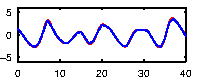
\includegraphics[width=0.48\textwidth]{Fig-LL0Jmf}
\caption{Lagrange wave in time with slight front-back asymmetry.}
\label{Fig1}
\end{SCfigure}

Figure~\ref{Fig1} shows a Lagrange time wave sampled at 1\,Hz in blue and a spline smoothed version in red.  The parameter {\tt lalpha} with value $1$ gives the waves a slightly steeper increase phase than decrease phase. The water depth is  {\tt S.h=20} [m].

The horizontal process is completely determined by the vertical
process.\footnote{In the most general form of a Lagrange model,  extra independent random harmonics can be added to the terms in $x(t,u)$. } If $w(t,u)$ is given by
\eqref{2DGauss}, then
\begin{align}
x(t,u) &= \sum_{j=0}^N \sqrt{S_j  \Delta \omega}\, \rho_j R_j \cos (\kappa_j u - \omega _j t + \Theta _j + \theta_j), \label{2DLagrange}
\end{align}
where $\rho_j$ is called the  {\it amplitude response} and $\theta_j$ is the {\it phase response} or ``phase shift''.

\subsubsection*{The response functions}
\addcontentsline{toc}{subsubsection}{\numberline{}The response functions}
The horizontal process $x(t,u)$ is a {\it linear filtration} of the vertical process $w(t,u)$ and the filter is defined by a frequency/wavenumber dependent complex response function $$H(\omega) = \rho(\omega) e^{i \theta(\omega)}.$$
The amplitude and phase responses in \eqref{2DLagrange} are then obtained as
\begin{align*}
\rho_j &= \rho(\omega_j), \quad \theta_j = \theta(\omega_j).
\end{align*}

The response functions determine the non-Gaussian characters of the Lagrange waves, in particular crest-trough and front-back asymmetry.  In the standard Lagrange model the filter response is depth and frequency dependent, given by
\begin{align}
H_M(\omega) &= i \frac{\cosh (h\kappa)}{\sinh (h\kappa)}, \label{Miche}
\end{align}
leading to a frequency independent phase shift of $\pi/2$ between vertical and horizontal movements.
The subscript $M$ in \eqref{Miche} stands for {\it Miche waves}; see \cite{Miche1944Mouvements}.
This choice of response function results in waves with crest-trough asymmetry, with more peaked crests and
shallower troughs compared to the Gaussian waves. However, Miche waves a front-back statistically symmetric;  wave fronts and wave back distributions are mirror images of each other; \cite{Aberg2007Wave,AbergAndLindgren2008Height}.

In order to give wave  front-back asymmetry the response function must give a frequency dependent phase shift. In {\sc Wafo}L this is realized by adding a term $\alpha/\omega^2$ to the Miche response,
\begin{align}
H(\omega) &= H_M(\omega) + \frac{\alpha}{\omega^2}. \label{H}
\end{align}
This choice corresponds to a direct relation between the horizontal particle acceleration and the vertical height,
\begin{align}
\frac{\partial ^2 x(t,u)}{\partial t ^2}
&= \frac{\partial ^2 x_M(t,u)}{\partial t^2}
- \alpha \, w(t,u)\label{alphamodel1}
\end{align}
where $x_M(t,u)$ is the Miche solution;  \cite{,Lindgren2009Exact,Lindgren2010Slope,
LindgrenAndAberg2009First}.

\section{Generating Lagrange waves with {\sc Wafo}L}
The basic routines in {\sc Wafo}L for simulation of Lagrange waves are
{\tt spec2ldat} and {\tt ldat2lwav}.

\subsection{The simulation options}
The parameters for the simulations are set by an options structure.  The default option {\tt opt = simoptset} gives the result
{\small\begin{verbatim}
opt =

          Nt: 2048
          Nu: 2048
          Nv: []
          dt: 0.5000
          du: 0.5000
          dv: []
      lalpha: 0
       lbeta: 0
     ffttype: 'ffttime'
       iseed: 'shuffle'
    plotflag: 0
\end{verbatim}
}
\noindent
with number of time and space points,  the corresponding time and space steps, and the value of the $\alpha$ parameter in \eqref{H}, ($\beta$ is not used in this tutorial). The {\tt ffttype} determines the hierarchy in the simulation -- {\tt ffttime} uses the FFT routine in time, stepping over the different space values. The alternatives are {\tt fftspace} and {\tt ffttwodim}. The {\tt iseed} option {\tt shuffle} sets the random number generator to, just, random.

%The options can be changed by, e.g.,
%{\small\begin{verbatim}
%   opt = simoptset(opt,'Nt',256,'dt',0.125,'Nu',512,'lalpha',1,'iseed',123791)
%\end{verbatim}
%}
\subsection{Generating  the elementary processes}
\begin{SCfigure}[1][t]
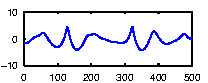
\includegraphics[width=0.48\textwidth]{Fig-FbAsymSpace1}
\caption{Front-back symmetric Lagrange space wave on shallow water {\tt (h = 8 m)}; direct plot.}
\label{Fig2}
\end{SCfigure}
The simulation routine {\tt spec2ldat} is an expansion of the {\sc Wafo} routines {\tt spec2sdat} and {\tt seasim}. Figure~\ref{Fig2} was generated by the following commands:
{\small\begin{verbatim}
   S = jonswap(1.5); S.h = 8;
   opt = simoptset('Nt',256,'dt',0.125,'Nu',256*8,'du',0.25,'iseed',123791);
   [w,x] = spec2ldat(S,opt,'iseed','shuffle') ; % Keep [w,x]
   subplot(211)
   plot(x.u+x.Z(:,128),w.Z(:,128));
   axis([0 500 -10 10]) % Keep the figure
\end{verbatim}
}
Note how {\tt simoptset} changes the default values of {\tt opt} and how  {\tt spec2ldat} resets seed option to {\tt 'shuffle'}.  The argument {\tt 1.5} in {\tt jonswap} is a cut off frequency to remove small ripples. The output {\tt [w,x]} gives the vertical and horizontal fields as structures with values at the selected space and time coordinates as fields {\tt 'Z','u','t'}:
{\small\begin{verbatim}
w =
       Z: [2048x256 double]
       u: [2048x1 double]
       t: [1x256 double]
    note: 'JONSWAP, Hm0 = 7, Tp = 11, gamma = 2.3853'

x =
        Z: [2048x256 double]
        u: [2048x1 double]
        t: [1x256 double]
    note1: 'Horizontal Lagrange component'
    note2: 'alpha=0, beta =0'
\end{verbatim}}
\noindent and the plot command  {\tt plot(x.u+x.Z(:,128),w.Z(:,128))} plots the space wave according to the definition, 
observed at time {\tt 16 = 128 * dt}.

\subsection{Generating the Lagrange wave}
The {\sc WafoL} routine {\tt ldat2lwav} is used to construct Lagrange time or space waves from the elementary 
processes. Keep the {\tt [w,x]} from the previous session and compute the space wave at time {\tt t0 = 16}:
{\small\begin{verbatim}
   [L,L0] = ldat2lwav(w,x,'space',16)
   subplot(212)
   plot(L.u,L.Z,L0.u,L0.Z,'r')
   axis([0 500 -10 10])
\end{verbatim}
}
The blue curve (almost invisible) in Figure~\ref{Fig3} is the same space wave as is plotted ``by hand'' in 
Figure~\ref{Fig2}. The red curve is a smoothed version; the two are almost identical.
The full call to the routine is
{\small\begin{verbatim}
   [L,Lsmooth]=ldat2lwav(w,x,type,tu0,dense)
\end{verbatim}
}
\noindent where {\tt type} can be {\tt 'time'} or {\tt 'space'} and {\tt tu0} is the space or time (in absolute units 
{\tt meter or seconds}), respectively, for which the wave is computed. The parameter {\tt dense} is the 
interpolation rate (a positive integer).
%{\tt removeloops} can be set to {\tt false} if one wants to keep possible loops in a space wave, but %there are no guarantees that it works properly at the moment.
The output {\tt Lsmooth} is an interpolated and smoothed version of {\tt L}; see also Subsection~\ref{loops} for exceptions where the Lagrange model give unphysical results.

 \begin{SCfigure}[1][t]
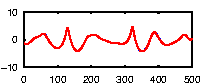
\includegraphics[width=0.48\textwidth]{Fig-FbAsymSpace2}
\caption{Front-back symmetric Lagrange space wave on shallow water {\tt (h = 8 m)} generated by {\tt ldat2lwav}.}
\label{Fig3}
\end{SCfigure}

\subsubsection*{The mean water level}
The Lagrange transformation acts on the Gaussian field $w(t,u)$ by compressing the crest parts of the waves, 
making them shorter in space or time, and expanding the trough parts, making them longer. This affects the 
empirical mean surface level and makes it (in general) negative. We illustrate this and take the mean of the 
Gaussian part and of the generated space Lagrange wave, and obtain, for the example above,
{\small\begin{verbatim}
   MGauss = mean(w.Z(:))
	MGauss = 1.2794e-16
   MLagrange = mean(L0.Z)
	MLagrange = -0.5025
\end{verbatim}}

\subsubsection*{The standard deviation}
\addcontentsline{toc}{subsubsection}{\numberline{}The standard deviation}

The distortion of the Gauss field also affects the standard deviation, making it smaller for the Lagrange wave 
than for the Gauss wave. The theoretical standard deviation for the Gaussian wave is obtained by the 
commands {\tt mom=spec2mom(S)} and {\tt std = sqrt\{mom(1)\}}. Our simulation yielded
{\small\begin{verbatim}
   SGauss = std(w.Z(:))
	SGauss = 2.0529
   SLagrange = std(L0.Z)
	SLagrange = 1.9376
\end{verbatim}
}
\noindent
For crest-trough asymmetric waves with peaked crests and flat troughs is it a general rule that the ratio between 
standard deviation and average crest-trough wave height is smaller than for a corresponding Gauss field.
\subsection{Depth dependence and loops}\label{loops}

The Lagrange transformation is  sensitive to the water depth. For infinite water depth the water particle will move in randomly perturbed circles. For decreasing depth the particle paths will be more and more elongated and randomly deformed ellipses, \cite{Miche1944Mouvements}. For very small depths the model may produce typical loops at the wave crests, where the water surface is folded. This is a consequence of the absence of physical constraints in the model.

The interpolation and smoothing in the {\sc Wafo}
routine {\tt ldat2lwav} does not accept loops and will produce a smoothed version  {\tt  Lsmooth}
up to about a wave period/wave length before the first loop. If the first loop occurs early in the series, then {\tt L0} will be empty.
The routine {\tt looptest(S,opt)} simulates independent samples of {\tt [w,x]} and gives as output the observed number of {\tt x}-fields in which loops has occurred.

The depth dependence for space waves is illustrated in Figure~\ref{Fig4},
generated by the following code -- to get time waves, just change the type option from {\tt 'space'}  to {\tt 'time'} and plot with {\tt L0.t}, etc. Note that the shallow water case {\tt S.h=3} will easily produce folding. In the plot we therefore use a direct plot routine for that case.
{\small\begin{verbatim}
   opt = simoptset('Nt',128,'Nu',2048,'du',0.25);
   S = jonswap(1.5);   S3 = S; S3.h = 3;
   S8 = S; S8.h = 8;   S32 = S; S32.h = 32;
   [w,x] = spec2ldat(S,opt);
   [w3,x3] = spec2ldat(S3,opt);
   [w8,x8] = spec2ldat(S8,opt);
   [w32,x32] = spec2ldat(S32,opt);
   [L,L0] = ldat2lwav(w,x,'space');
   [L3,L03] = ldat2lwav(w3,x3,'space');
   [L8,L08] = ldat2lwav(w8,x8,'space');
   [L32,L032] = ldat2lwav(w32,x32,'space');

   figure(1);    clf
   subplot(411)
   plot(L0.u,L0.Z); axis([0 500 -5 5]);
   title('Depth = \infty')
   subplot(412)
   plot(L032.u,L032.Z); axis([0 500 -5 5]);
   title('Depth = 32 m')
   subplot(413)
   plot(L08.u,L08.Z); axis([0 500 -5 5]);
   title('Depth = 8 m')
   subplot(414)
   % 3m water depth may cause loops and ldat2lwav
   % then gives only a short piece of L03.
   % We plot space wave directly from w3,x3 as in Figure 1.2
   plot(x3.u+x3.Z(:,64),w3.Z(:,64))
   axis([0 500 -5 5])
   title('Depth = 3 m')
\end{verbatim}
}

 \begin{SCfigure}[1][t]
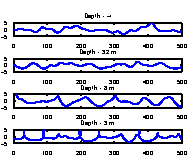
\includegraphics[width=0.48\textwidth]{Fig-CtAsymSpaceDepth}
\caption{Crest-trough asymmetric Lagrange space wave on different water depth.}
\label{Fig4}
\end{SCfigure}

\noindent
Figure~\ref{Fig4b}  shows the truncation effect of {\tt ldat2lwav} with the following code.
{\small\begin{verbatim}
   S=jonswap(1.5); S.h=20;
   opt=simoptset('dt',0.125,'lalpha',2);
   [w,x]=spec2ldat(S,opt);
   [L,L0]=ldat2lwav(w,x,'time',[],10,1)
   pause
   S=jonswap(1.5); S.h=4;
   opt=simoptset('dt',0.125,'lalpha',0,'ffttype','fftspace');
   [w,x]=spec2ldat(S,opt);
   [L,L0]=ldat2lwav(w,x,'space',[],10,1)
\end{verbatim}
}
\noindent
If no {\tt subplot(212)} appears, {\tt L0} was empty -- try again.

\begin{figure}
\centerline{
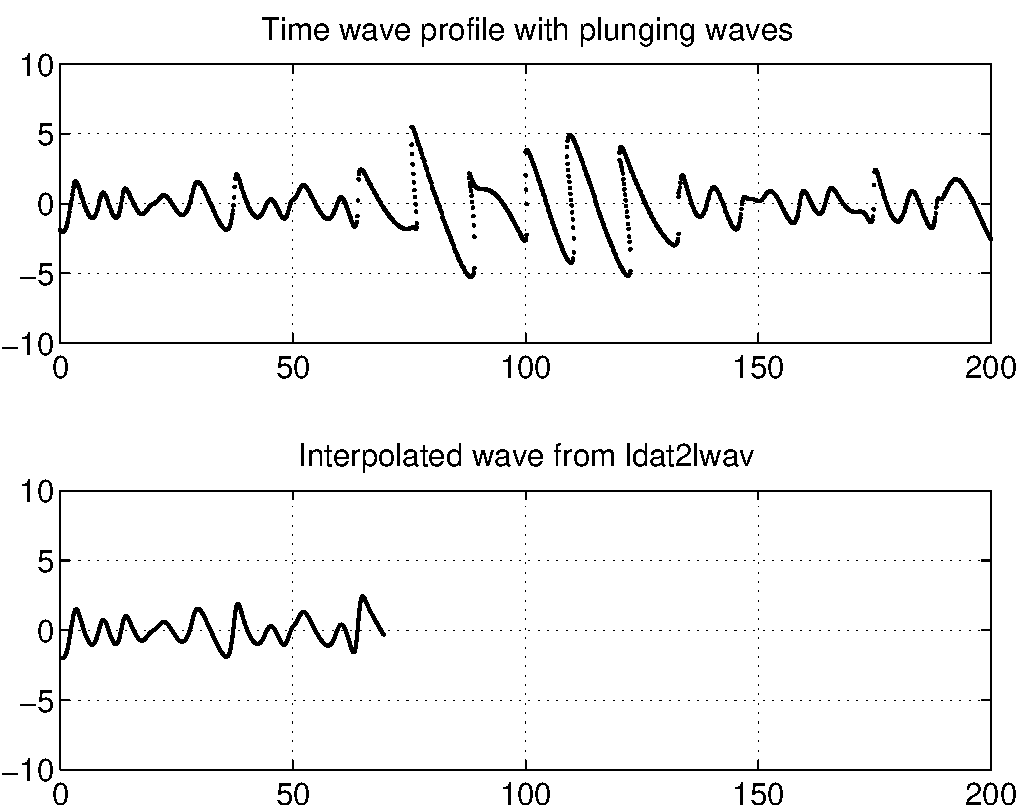
\includegraphics[width=0.45\textwidth]{Fig-FoldingTime-a}
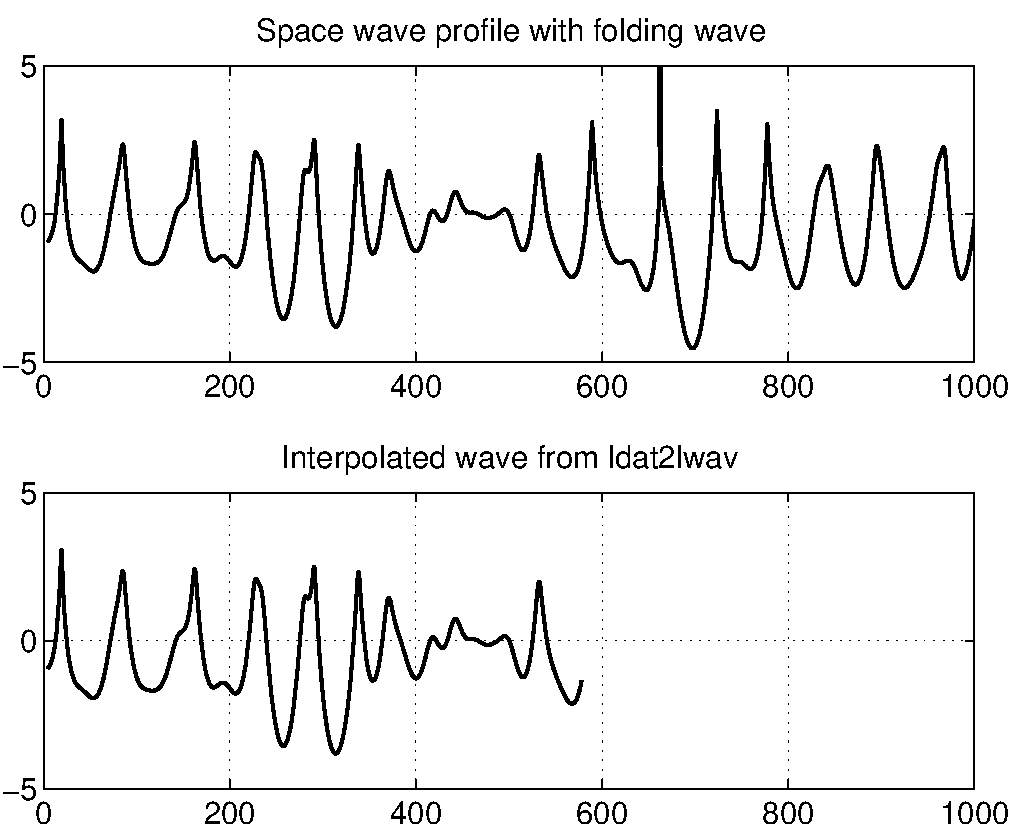
\includegraphics[width=0.45\textwidth]{Fig-FoldingTime-b}
}
\caption{Left: Time wave profile with plunging wave truncated by {\tt ldat2lwav}.
Right: Space wave profile with folded wave truncated by {\tt ldat2lwav}.}
\label{Fig4b}
\end{figure}

\subsection{Front-back asymmetry}\label{ss:frontbackasymmetry}
The main feature of the Lagrange approach is that it can easily generate waves with realistic front-back asymmetry.\footnote{The crest-trough asymmetry generated by the Lagrange transformation can also be found in the 2$^{nd}$ order Stokes waves; see 
Chapter~\ref{Secondorderwaves}.}
The asymmetry is controlled by the parameter {\tt opt.lalpha}.
This example illustrates, in Figure~\ref{Fig5},  the effect of different $\alpha$-values on the front-back asymmetry,

{\small\begin{verbatim}
   opt = simoptset('Nt',2048,'dt',0.125,'Nu',512,'du',0.25);
   S = jonswap(1.5); S.h=20;
   [w0,x0] = spec2ldat(S,opt);
   [w1,x1] = spec2ldat(S,opt,'lalpha',0.75);
   [w2,x2] = spec2ldat(S,opt,'lalpha',1.5);
   [L0,L00] = ldat2lwav(w0,x0,'time');
   [L1,L01] = ldat2lwav(w1,x1,'time');
   [L2,L02] = ldat2lwav(w2,x2,'time');
   figure(1); clf
   subplot(311); plot(L00.t,L00.Z);title('\alpha = 0');
   axis([0 50 -10 10])
   subplot(312); plot(L01.t,L01.Z);title('\alpha = 0.75');
   axis([0 50 -10 10])
   subplot(313); plot(L02.t,L02.Z);title('\alpha = 1.5');
   axis([0 50 -10 10])
 \end{verbatim}
}
\noindent Note that Figure~\ref{Fig5} shows time waves where the steep wave side is facing left. You should generate the corresponding space waves -- then you can chose
a smaller {\tt Nt} and a larger {\tt Nu}-value.
 \begin{SCfigure}[1][t]
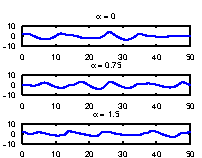
\includegraphics[width=0.48\textwidth]{Fig-FbAsymTimeAlpha}
\caption{Front-back asymmetric Lagrange time waves with different $\alpha$-values. Water depth:  {\tt S.h = 20[m]}. }
\label{Fig5}
\end{SCfigure}
\section{Slopes and asymmetry measures}
\subsubsection*{An argument for the Gauss-Lagrange model}
\addcontentsline{toc}{subsubsection}{\numberline{}An argument for the Gauss-Lagrange model}

To be really useful in practice any physical,  mathematical or stochastic wave model has to be calibrated against empirical data. The stochastic Gauss-Lagrange wave model offers unique features, not shared by deterministic models, which can be used for calibration. Some of these features are also useful in their own right, and most important of these are the statistical distributions of different geometrical wave characteristics.

\subsection{Extracting slope characteristics from wave data}\label{ss:extracting}
{\sc Wafo}L offers two ways to extract slope values from wave data, one general and one based on the special Lagrange format with separate vertical and horizontal components.

The general routine
{\tt wav2slope} can be applied to all types of wave data with the call
{\small\begin{verbatim}
   Slopes = wav2slope(L,absolutelevels,dense,p)
\end{verbatim}
}
\noindent
It takes a time or space wave {\tt L} and extracts slope values at  up- and downcrossings of the levels defined by the vector {\tt absolutelevels}, after interpolation with rate {\tt dense} and smoothing with parameter {\tt p} with default value {\tt p = 1}. The wave data {\tt L} must be a structure with values in {\tt L.Z} and arguments in {\tt L.t} or {\tt L.u}, for time and space waves, respectively. The arguments must be in increasing order, but need not be equidistant.

The second route is intended for simulated Lagrange wave data and it uses the basic structure of the model. The call is
{\small\begin{verbatim}
   Slopes = ldat2lslope(w,x,type,absolutelevels)
\end{verbatim}}
\noindent Here {\tt w, x} are the output of the simulation routine {\tt spec2ldat}. This routine identifies the {\tt x}- and {\tt w}-combinations that generate a time or space wave and computes the slope according to
equations (9) and (10) in \cite{Lindgren2010Slope}. It disregards crossings that are combined with folding of plunging waves.

A special routine is available for simulation experiments with slope distributions directly from the orbital spectrum {\tt S}.  The call
{\small\begin{verbatim}
   Slopes = spec2slopedat(S,Nsim,type,relativelevels,opt)
\end{verbatim}}
\noindent simulates {\tt Nsim} independent samples of Lagrange waves with specified spectrum and extracts the slopes, using {\tt wav2slope}.
The default choice of levels is {\tt relativelevels = [-1 0 1 2]}
which will give slopes at crossing of the absolute levels {\tt [-1 0 1 2]*Hs/4}
relative to the still water level {\tt mwl = 0}; note {\tt Hs = 4*std}.
The routine {\tt spec2steepdat} is an extension of {\tt spec2slopedat} and it will be described in
Section~\ref{ss:asymmetrymeasures}.

\subsubsection*{Empirical slope distribution}
\addcontentsline{toc}{subsubsection}{\numberline{}Empirical slope distribution}

To illustrate slope distributions in front-back asymmetric wave data we first generate synthetic waves and then
use the first routine on the data. We use the same models as for Figure~\ref{Fig5} and  extract the slopes at the up- and downcrossings of levels {\tt [0 1 2]*std} defined in units of standard deviations relative to the still water level. The call
{\small\begin{verbatim}
   opt = simoptset('Nt',2048*16,'dt',0.125,'Nu',512,'du',0.25);
   S = jonswap(1.5,[6 10]); S.h=20;
   [w0,x0] = spec2ldat(S,opt);
   [w1,x1] = spec2ldat(S,opt,'lalpha',0.5);
   [w2,x2] = spec2ldat(S,opt,'lalpha',1);
   [L0,L00] = ldat2lwav(w0,x0,'time');
   [L1,L01] = ldat2lwav(w1,x1,'time');
   [L2,L02] = ldat2lwav(w2,x2,'time');
   mom = spec2mom(S);
   levels=[0 1 2]*sqrt(mom(1)); % wav2slope requires absolute levels
   Slope0 = wav2slope(L00,levels);
   Slope1 = wav2slope(L01,levels);
   Slope2 = wav2slope(L02,levels)
\end{verbatim}
}
\noindent
will produce a result like (depending on the randomness)
{\small\begin{verbatim}
Slope2 =

        up: {[993x1 double]  [560x1 double]  [110x1 double]}
      down: {[993x1 double]  [560x1 double]  [110x1 double]}
    levels: [0 1.4800 2.9600]
\end{verbatim}
}
The plot the empirical distributions in Figure~\ref{Fig16} of the slopes of the mean level we use the
{\sc Wafo} routine {\tt plotedf},
{\small\begin{verbatim}
   plotedf(Slope0.up{1}); hold on
   plotedf(Slope1.up{1});
   plotedf(Slope2.up{1});
   plotedf(-Slope0.down{1},'r-.')
   plotedf(-Slope1.down{1},'r-.');
   plotedf(-Slope2.down{1},'r-.');
   axis([0 8 0 1])
\end{verbatim}
}

\begin{SCfigure}[1]
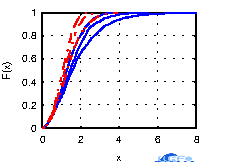
\includegraphics[width=0.48\textwidth]{Fig-SlopeCDFTimeAlpha}
\caption{Empirical distributions of up- an downcrossing (absolute values) slopes at still water level for Lagrange time waves with different degrees of front-back asymmetry; $\alpha = 0, 0.5, 1$.}
\label{Fig16}
\end{SCfigure}

Simulated slope distributions can be generated directly from the spectrum by the routine {\tt spec2slopedat}. As a by-product we also get the average shape of the waves in the neighbourhood of upcrossings and downcrossings of the mean waterlevel. We generate some such empirical distributions before we compute the exact theoretical ones. Figure~\ref{Fig1.7} shows, in the upper row, simulated CDF of slopes at up- and downcrossings of different levels.  The lower row shows the average wave shape near up- and downcrossing of the mean water level. (The downcrossing curves are mirrored in the origin to be comparable with upcrossings ditto.)  First compute the distributions,

{\small\begin{verbatim}
   S=jonswap(1.5,[6 10]); S.h=20;
   opt=simoptset(opt,'Nt',64,'dt',0.25,...
        'Nu',2048*16,'du',0.25,'ffttype','fftspace');
   Nsim=100; % Takes time; Nsim = 10 in the command script
   Slopes=spec2slopedat(S,Nsim,'space',[],opt)
   Slopes1=spec2slopedat(S,Nsim,'space',[],opt,'lalpha',1)
\end{verbatim}
}
\noindent
and then plot the empirical CDF:s and the average waves; Fig~\ref{Fig1.7}.
{\small\begin{verbatim}
   figure(1);   clf
   subplot(221);  box; hold on
   for f=1:length(Slopes.levels),
      if ~isempty(Slopes.up{f}
         plotedf(Slopes.up{f})
      end
      if ~isempty(Slopes.down{f})
         plotedf(-Slopes.down{f},'-.')
      end
   end
   axis([0 0.8 0 1])
   subplot(222);  box; hold on
   for f=1:length(Slopes1.levels),
      if ~isempty(Slopes1.up{f})
         plotedf(Slopes1.up{f})
      end
      if ~isempty(Slopes1.down{f})
         plotedf(-Slopes1.down{f},'-.')
      end
   end
   axis([0 0.8 0 1])
   subplot(223);  box;  hold on
   plot(Slopes.meanwavex,Slopes.meanwaveup); ax=axis;
   axis([Slopes.meanwavex(1) Slopes.meanwavex(end) ax(3) ax(4)])
   plot(Slopes.meanwavex,Slopes.meanwavedown,'-.'); grid
   subplot(224);  box;  hold on
   plot(Slopes1.meanwavex,Slopes1.meanwaveup)
   axis([Slopes.meanwavex(1) Slopes.meanwavex(end) ax(3) ax(4)])
   plot(Slopes1.meanwavex,Slopes1.meanwavedown,'-.'); grid
\end{verbatim}
}
\begin{figure}[h]
\centerline{
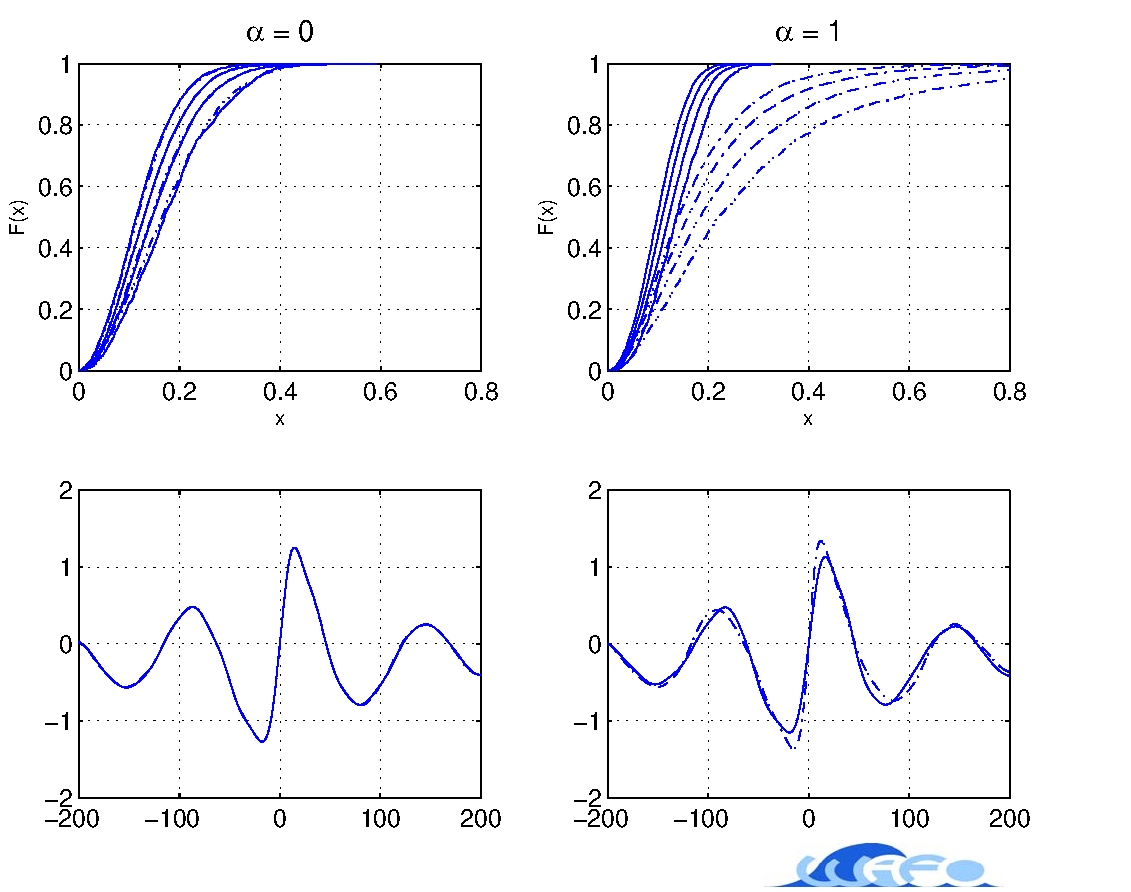
\includegraphics[width=0.72\textwidth]{Fig-SlopeAverageSpaceAlpha_b}
}
\caption{Space waves. Upper row: Simulated CDF of slopes at up (solid) and down (dash-dotted)  crossings of levels {\tt [-1 0 1 2]*standard deviation}. Left: front-back symmetric waves, $\alpha = 0$, where up- and downcrossing profiles are identical. Right: asymmetric waves, $\alpha = 1$. Lower row: Average wave shape near up- (solid) and down- (dash-dotted) crossings.}
\label{Fig1.7}
\end{figure}

One can see from the upper left plot in Figure~\ref{Fig1.7} that the slopes become steeper
with increasing level, in agreement with the crest-trough asymmetry of the Lagrange waves.


Simulation with {\tt lalpha > 1} may generate warnings for double crossings
(= folding waves) and empty output. Such waves are discarded in the simulation which
means that the generated slopes are slopes in waves where no folding occurred.
Each repetition in the example corresponds to {\tt 8192 m} of waves,
and in a run with 400 repetitions with $\alpha = 1.5$ a total of 34 fields were
discarded.\footnote{The reason to disregard folded waves is that slope distribution
becomes less meaningful for such waves.}
To obtain sufficient accuracy, 50 repetitions are sufficient.

Run a similar example with time waves with a larger {\tt opt.Nt} and smaller
{\tt opt.Nu} -- see code in {\sc Wafo}L.m.
Notice how downcrossing slopes are smaller than the upcrossing
ones for time waves, while the opposite holds for space waves.

\subsection{Theoretical slope distribution}\label{ss:TheoreticalSlopeDistributions}
The {\sc Wafo}L module contains routines for computation of the exact theoretical slope distribution at level crossings, based on the crossing theory in \cite{Lindgren2009Exact,Lindgren2010Slope}.

The main routines to get the exact theoretical slope distribution CDF:s directly from  the orbital
spectrum are {\tt spec2timeslopecdf} and {\tt spec2spaceslopecdf} and the related routines for the PDF-functions. We can now compare the empirical slop distributions that we just obtained with the theoretical ones.

We use the observed (simulated) {\tt Slopes1} values from the previous example and compare with the theoretical distribution. For time waves we use the following commands. First, simulate slopes:
{\small\begin{verbatim}
   S=jonswap(1.5,[6 10]); S.h=20;
   opt=simoptset('Nt',2048*16,'dt',0.125,...
        'Nu',128,'du',0.25,'ffttype','ffttime');
   Nsim=100; % Takes time; {\tt Nsim = 10} in the command script
   lev=[-1:2];  % Relative levels
   % Absolute levels will be computed from spectral moment
   Slopes=spec2slopedat(S,Nsim,'time',lev,opt)
   Slopes1=spec2slopedat(S,Nsim,'time',lev,opt,'lalpha',1)
\end{verbatim}
}
\noindent
Then compute the theoretical CDF:s,
{\small\begin{verbatim}
   y=0:0.01:10;
   [Fu,Fd] = spec2timeslopecdf(S,y,lev,opt);
   [Fu1,Fd1] = spec2timeslopecdf(S,y,lev,opt,'lalpha',1);
\end{verbatim}
}
\noindent
and compare the results for $\alpha = 1$ in Figure~\ref{TheorEmp} (for code, see {\tt WafoLCh1.m}).
\begin{SCfigure}[1.2]
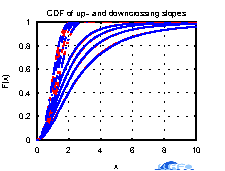
\includegraphics[width=0.45\textwidth]{Fig-CDFTimeTheorEmp_b}
\caption{CDF for up- and downcrossing (absolute values) slopes in asymmetric time waves with asymmetry parameter 
$\alpha=1$:
red = theoretical, blue = simulated, solid = upcrossing, dash-dotted = downcrossing. Crossed levels =
{\tt [-1 0 1 2]*standard deviation}. Outer curves = highest level.
}
\label{TheorEmp}
\end{SCfigure}

\subsection{Asymmetry measures}\label{ss:asymmetrymeasures}
Wave asymmetry and wave steepness can be summarised in many different ways,
and many measures have been suggested in the literature.
To define the measures we need to define some geometric wave characteristics.
With notations as in Figure~\ref{FigDefinitions}, we define for {\it time waves},
\begin{description}
\item[Slope ratio at down/up-crossings:] $\lambda_{AL} = -\frac{{\sf E}(L_t(t_{down}))}{{\sf E}(L_t(t_{up}))}
\approx \frac{{\sf E}(H_{cb}/T_{cb})}{{\sf E}(H_{cf}/T_{cf})}$, \label{LAL}
\item[Front/back period ratio:] $\lambda_{NLS} = {\sf E}(T_{cf})/{\sf E}(T_{cb}),$ \label{LNLS}
\item[Hilbert transform:] $A_H = {\sf E}(\widehat L (t)^3)/\sigma^3$. \label{AH}
\end{description}

\begin{figure}[tbh]
\centerline{
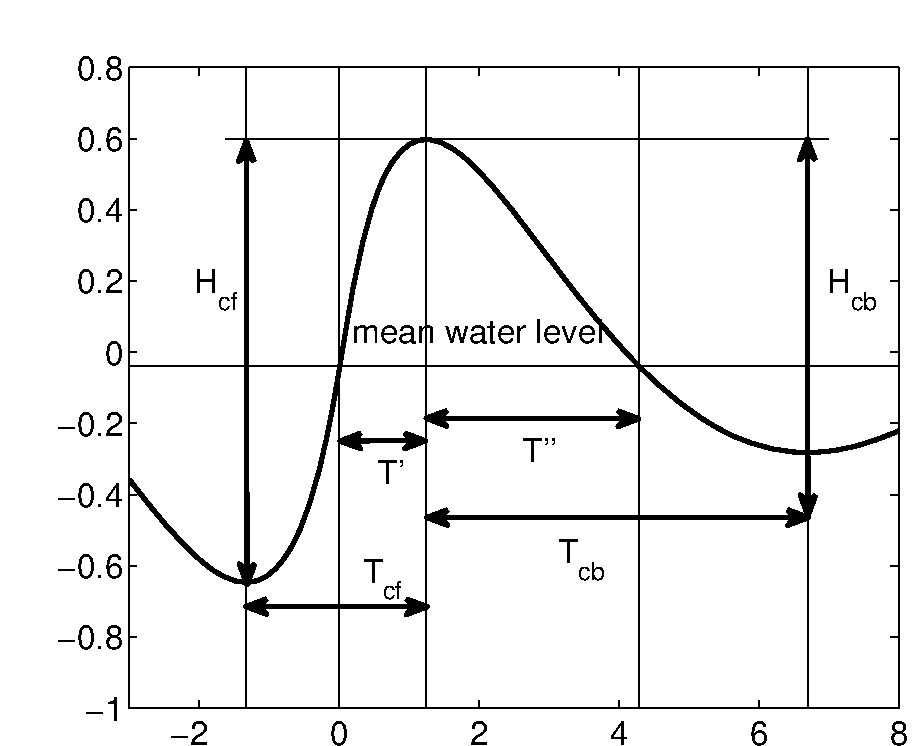
\includegraphics[width=0.46\textwidth]{Timewavedefinitions_b}
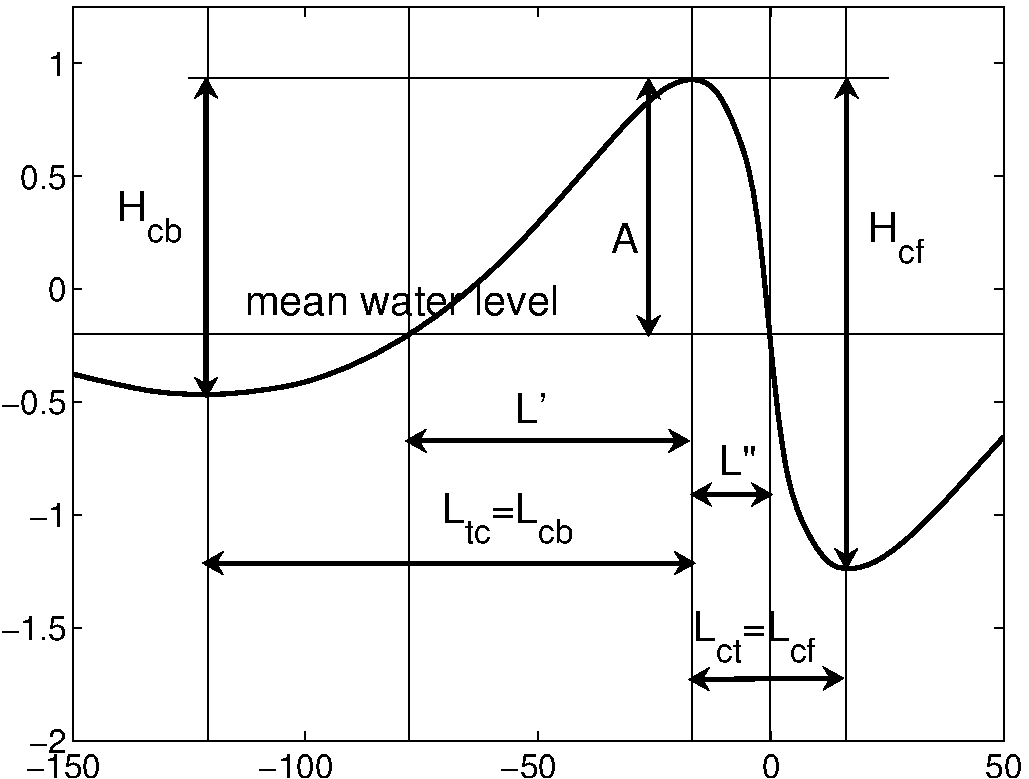
\includegraphics[width=0.454\textwidth]{Spacewavedefinitions}
}
\caption{Asymmetry characteristics for time (left) and space (right) waves moving from left to right.
The subscripts {\tt cb,cf} refer to crest-back and crest-front definitions,
and the subscripts {\tt tc,ct} refer to trough-crest and crest-trough definitions.}
\label{FigDefinitions}
\end{figure}

The measure $\lambda_{AL}$ was defined in \cite{LindgrenAndAberg2009First} and is based on
the slopes $L_t(t_{down})$ and $L_t(t_{up})$ at down- and upcrossings of the mean level.
If front and back crest amplitudes are about the same, it is approximately equal to the index
$\lambda_{NLS}$, proposed in \cite{NiedzweckiEtal1999}. The third measure $A_H$, introduced 
in \cite{LeykinEtal1995}, is based on the Hilbert transform $\widehat L (t)$ and is defined from 
its third moment and standard deviation.

The three asymmetry measures can be computed by simulation from the spectrum by the
{\sc Wafo}L routine {\tt spec2steepdat} with the call
{\small\begin{verbatim}
   [Slope, Steep, Data] = spec2steepdat(S,Nsim,type,relativelevels,opt)
\end{verbatim}
}
\noindent
The routine is an extended (and more time-consuming) version of  {\tt spec2slopedat}, the routine
that we used in Section~\ref{ss:extracting}.
It generates, besides the slope characteristics at level crossings, crest front/back period data, and a data structure with simulated Lagrange data, together with first and second derivatives.

The structure {\tt Slope} has fields with indices {\tt lambdaAL} and {\tt AH}, while the index {\tt lambdaNLS} is a field in {\tt Steep}. The following time consuming commands were used to generate the asymmetry data in Table~\ref{Tab11}. You may want to experiment with a smaller (or larger!) {\tt Nsim}.
{\small\begin{verbatim}
   S = jonswap(1.5,[6 10]); S.h=20;
   opt = simoptset('Nt',2048*16,'dt',0.125,...
        'Nu',321,'du',0.125,'ffttype','ffttime');
   Nsim = 50; % Change this to  Nsim = 10 or 20
   [Slope0,Steep0,~] = spec2steepdat(S,Nsim,'time',[],opt);
   [Slope05,Steep05,~] = spec2steepdat(S,Nsim,'time',[],opt,'lalpha',0.5);
   [Slope10,Steep10,~] = spec2steepdat(S,Nsim,'time',[],opt,'lalpha',1);
   [Slope15,Steep15,~] = spec2steepdat(S,Nsim,'time',[],opt,'lalpha',1.5);
   [Slope20,Steep20,~] = spec2steepdat(S,Nsim,'time',[],opt,'lalpha',2.0);
\end{verbatim}
}
The $\lambda$-indices in Table~\ref{Tab11} are easy to interpret. For example,
$\lambda_{AL} = 0.529$ for $\alpha = 1$ means that the time wave rate of
increase is about twice as fast as the decrease at the still water level. The value $\lambda_{NLS} = 0.552$ for $\alpha = 2$ means that the time crom trough to crest is about half the time from crest to trough, on average.
\begin{SCtable}[0.9][h]
\begin{tabular}{|l|ccc|}\hline
& $\lambda_{AL}$ & $\lambda_{NLS}$ & $A_H$ \\ \hline
$\alpha = 0.0$ & 1.005 & 1.002 & 0.005 \\
$\alpha = 0.5$ & 0.737 & 0.855 & -0.191 \\
$\alpha = 1.0$ & 0.529 & 0.734 & -0.386 \\
$\alpha = 1.5$ & 0.350 & 0.630 & -0.588 \\
$\alpha = 2.0$ & 0.226 & 0.552 & -0.644 \\ \hline
\end{tabular}
\caption{Simulated asymmetry measures in time waves for different $\alpha$-values.}
\label{Tab11}
\end{SCtable}


\chapter{3D Lagrange waves}\label{3DLagrangeWaves}
\section{The 3D Lagrange  model}
The 3D Lagrange model consists of a Gaussian homogeneous random field $w(t,u,v)$ for the vertical movements of water particles and two correlated Gaussian fields $x(t,u,v) , y(t,u,v)$ for the horizontal movements. The total energy of $w(t,u,v)$  is distributed over elementary waves with frequency $\omega$ and direction $\theta$ according to a {\it directional orbital spectrum} $S(\omega, \theta)$, $\omega > 0$, $-\pi < \theta \leq \pi$. The $x$-process describes the horizontal movements in the directions $\theta = 0, \pi$, and $y$ the movements in the directions $\theta = \pm \pi/2$.

For simulation purposes in {\sc Wafo}L the spectrum is discretized over wave-numbers $\kappa^u_{jk}$, $\kappa^v_{jk}$, and with related frequencies
$\omega_{jk} > 0$, given by the dispersion relation,
$$
\omega^2 = g |\kappa| \tanh h |\kappa|, \quad |\kappa| = \sqrt{\kappa_u^2 + \kappa_v^2}.
$$

In analogy with \eqref{2DGauss} and \eqref{2DLagrange} the three components in the 3D model are
\begin{align}
w(t,u,v) &=
\sum_{j,k} \sqrt{S_{jk}}\, R_{jk} \cos (\kappa^u_{jk} u + \kappa^v_{jk} v - \omega _{jk} t
+ \Theta _{jk}), \label{3DGauss} \\
x(t,u,v) &=
\sum_{j,k} \sqrt{S_{jk}}\, R_{jk} \, \rho^u_{jk} \cos (\kappa^u_{jk} u + \kappa^v_{jk} v - \omega _{jk} t
+ \Theta _{jk} + \psi ^u_{jk}),
\label{3DX} \\
y(t,u,v) &=
\sum_{j,k} \sqrt{S_{jk}}\, R_{jk} \, \rho^v_{jk} \cos (\kappa^u_{jk} u + \kappa^v_{jk} v - \omega _{jk} t
+ \Theta _{jk} + \psi ^v_{jk}),
\label{3DY}
\end{align}
\subsubsection*{The 3D Lagrange wave field}
\addcontentsline{toc}{subsubsection}{\numberline{}The 3D Lagrange wave field}
The 3D lagrange wave field is a random time varying field $L(t; x, y), t \in \mR, (x,y) \in \mR^2$ that, at time $t$, takes the value $w(t,u,v)$ at location $(x=x(t,u,v), y=y(t,u,v)$:
\begin{align}
L(t; x(t,u,v), y(t,u,v)) &= w(t,u,v). \label{L}
\end{align}
It may happen that there are more than one $(u,v)$ for which $(x(t,u,v), y(t,u,v) ) =(x,y)$; in that case $L$ takes multiple values.

\subsubsection*{The response functions}
\addcontentsline{toc}{subsubsection}{\numberline{}The response functions}

The response functions are allowed to depend on frequency $\omega$ and direction $\theta$,  and wave-number $\bkappa = (\kappa ^u, \kappa ^v) $ as in the 2D case. Now, there is more freedom to introduce asymmetry, depending on wave direction, and the user  can construct a model for any special purpose. The standard implementation of {\sc Wafo}L uses the following generalization of \eqref{H}, introduced in \cite[Eqn. (10)]{LindgrenAndLindgren2011Stochastic},
\begin{align}
\bH(\theta, \bkappa) &=
\begin{pmatrix}
\rho^u e^{i \psi^u} \\
\rho^v e^{i \psi^v}
\end{pmatrix} =
\frac{\alpha}{\omega^2}\! \cdot \! \begin{pmatrix}
 \cos^2 (\theta)\, |\cos (\theta)| \\
\cos^2(\theta) \sin (\theta) \sign(\cos \theta)
\end{pmatrix}
+ i \frac{\cosh |\bkappa| h}{\sinh |\bkappa| h} \! \cdot \!
\begin{pmatrix}\cos \theta \\ \sin \theta \end{pmatrix}.
\label{specialtransfer}
\end{align}
This choice modifies the front-back asymmetry for waves with direction away from $\theta = 0, \pi$ and blocks it completely at $\theta = \pm \pi/2$.

\section{Generating 3D Lagrange waves with {\sc Wafo}L}
\subsection{Generating the elementary processes by {\tt spec2ldat3D}}
{\sc Wafo}L offers two routines for simulation of the 3D 
elementary processes, and 
in this chapter we describe the 1$^{st}$ order routine, {\tt spec2ldat3D}. 
The alternative routine is called {\tt spec2ldat3DM} and it can also generate 
non-linear, 2$^{nd}$ order Stokes variation, both in vertical and horizontal dimension. 
That routine and its parallel companion {\tt spec2ldat3DP} will be described in Chapter~\ref{Secondorderwaves}. 

\subsubsection*{The directional spectrum}
\addcontentsline{toc}{subsubsection}{\numberline{}The directional spectrum}

The most important input variable is of course the directional orbital 
power spectrum for the Gaussian wave field $w(t,u,v)$.
 It can be given it either frequency-direction form or in wave-number
 form, both supported by  {\sc Wafo} and {\sc Wafo}L. 

The simplest way to produce a directional spectrum is illustrated by 
the example  in the {\sc Wafo}-routine {\tt mkdspec},
{\small\begin{verbatim}
   S = jonswap
   D = spreading(linspace(-pi,pi,51),'cos2s')
   Snew = mkdspec(S,D,1)
\end{verbatim}}
\noindent
that will produce the left plot in Figure~\ref{Dspec_dir}. The wave-number spectrum to the right is produced by
{\small\begin{verbatim}
   Sk2d = spec2spec(Snew,'k2d')
   plotspec(Sk2d)
   axis([-0.05 0.05 -0.05 0.05])
\end{verbatim}
}

The general form of the {\tt spreading} command is
{\small\begin{verbatim}
   D = spreading(directions,type,maindirection,spreading,frequencies,fdep)
\end{verbatim}
}
\noindent
For experiments with front-back asymmetry it is recommended to set {\tt maindirection = 0}. 
The parameter {\tt spreading} defines the degree of directional spreading; {\tt spreading = 0} 
gives isotropic waves with equal energy in all directions, a high value gives almost uni-directional 3D 
waves moving from ``right to left'' -- this convention differs from that in 
Section~\ref{ss:gauss}. \label{wavedirection}
The default value is {\tt spreading = 15} as in the example. Observe that {\tt frequencies} 
must be the same as the frequencies in the spectrum, {\tt S.w}; the standard spectra in 
{\sc Wafo} have the same default values as the {\tt spreading} function. The last 
parameter, {\tt fdep} takes values $0, 1$ for frequency independent or frequency 
dependent spreading (default), respectively. 
\begin{figure}[tbh]
\centerline{
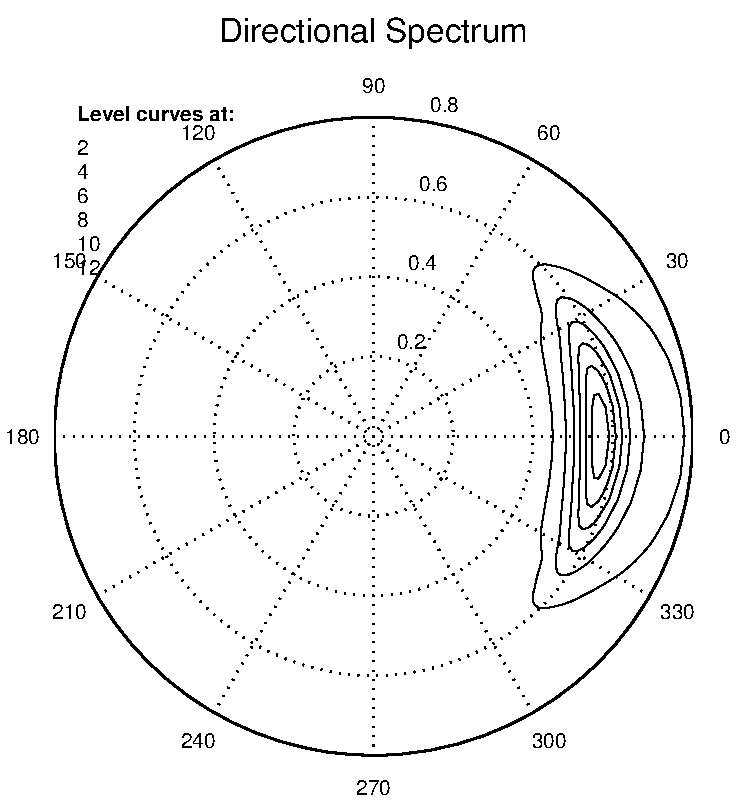
\includegraphics[width=0.31\textwidth]{Fig_Dspec_dir_a}
\hspace{5mm}
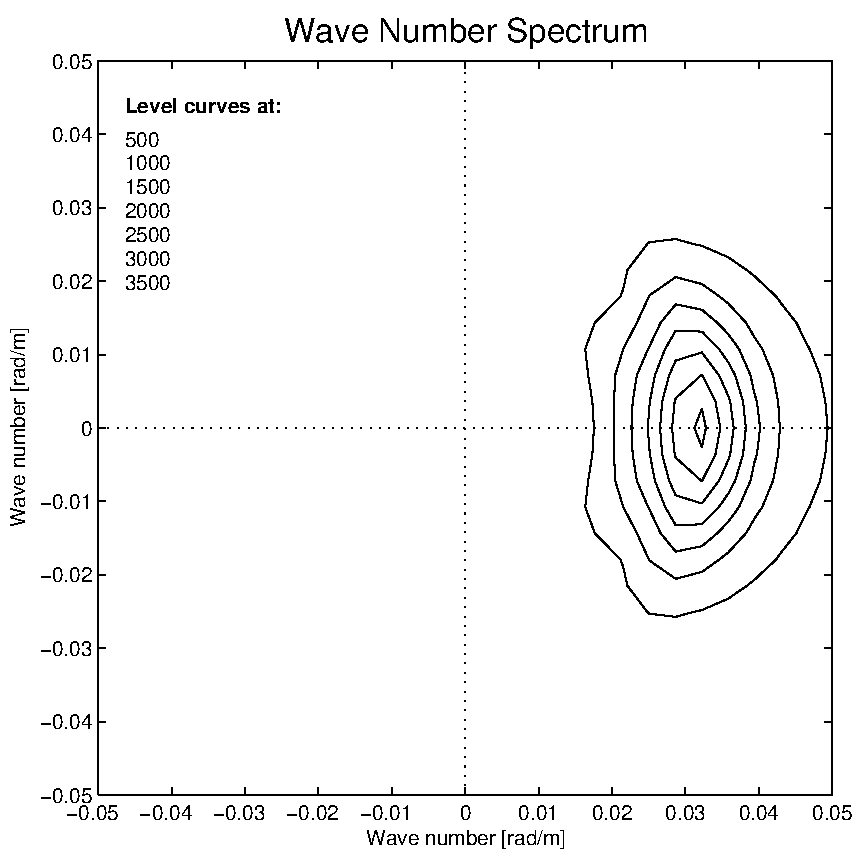
\includegraphics[width=0.34\textwidth]{Fig_Dspec_k2d}
}
\caption{Left: directional spectrum in frequency-direction form. Right: the same spectrum in wave-number form.}
\label{Dspec_dir}
\end{figure}

\subsubsection*{The simulation options in {\tt spec2ldat3D}}
\addcontentsline{toc}{subsubsection}{\numberline{}The simulation options}
The options command {\tt opt = simoptset} is used to define the number of time and space coordinates, {\tt Nt, Nu, Nv},  their spacings, {\tt dt, du, dv}, the asymmetry parameter {\tt lalpha}, the seed for the random number generator {\tt iseed}, (default {\tt shuffle}), and the {\tt plotflag}. The simulation in 
{\tt spec2ldat3D} is always done with a 2D FFT over space, 
then looping over time, so the {\tt ffttype} option is not relevant 
for the 3D model.
The simulation generates a large data set with three fields 
of size {\tt Nt x Nu x Nv} each, and there is a memory trade-off 
between time and space.

If one seeks a large wave field at only one time point, one can choose 
{\tt Nt = 1} and {\tt Nu, Nv} as large as needed.  But if the goal is to get 
a set of long wave time series, i.e. {\tt Nt} large, at a modest number 
of locations, one must be sure not to take {\tt Nu x Nv} too small, 
and this for two reasons. First, both {\tt Nu} and {\tt Nv} must be 
big enough to cover the full variation of the horizontal movements 
within the studied region. This means, for example, that if one 
wants to generate wave a field over an area of size {\tt 200x100 meters} 
then one should have {\tt Nu x du} at least\label{opt}
{\tt 200 + 6 std(X)} and similar for  the 
{\tt Y}-field.\footnote{{\tt std(X)} can be estimated by
{\tt mean(mean(std(X.Z)))}.}

Second, the number of space points defines in a non-systematic way the periodicity of the time waves. At present, there is no systematic study of how large space field is needed to avoid bias caused by time periodicity. The user is advised not to generate excessively long time series but rather generate many independent series. 

In the examples we use the following {\tt options} for time and space oriented problems:
{\small\begin{verbatim}
   optTime = simoptset('Nt',1001,'dt',0.2,...
                          'Nu',128,'du',5,'Nv',64,'dv',5);
   optSpace = simoptset('Nt',1,'dt',0.5,...
                          'Nu',1024,'du',1,'Nv',512,'dv',1);
\end{verbatim}
}

\subsubsection*{Generation of the elementary processes}
\addcontentsline{toc}{subsubsection}{\numberline{}Generation of the elementary processes}
The elementary processes are generated by the routine {\tt spec2ldat3D}.
First we define the directional spectrum and then generate the elementary processes.
We define two spreading functions, one, {\tt D5}, that gives moderate spreading,
and one, {\tt D15}, that gives waves with more concentrated direction.

{\small\begin{verbatim}
   S = jonswap(1.5); S.h = 20;
   D5 = spreading(101,'cos',0,5,S.w,0);
   SD5 = mkdspec(S,D5);
   D15 = spreading(101,'cos',0,15,S.w,0);
   SD15 = mkdspec(S,D15);
\end{verbatim}
}

\noindent
The time option
{\small\begin{verbatim}
   [W,X,Y] = spec2ldat3D(SD5,optTime);
\end{verbatim}
}
\noindent takes about 30 seconds and generates about 200 MB of wave data. The space option
{\small\begin{verbatim}
   [W,X,Y] = spec2ldat3D(SD5,optSpace);
\end{verbatim}
}
\noindent takes less than 1 second and generates about 25 MB of wave data.

\subsection{Generating the Lagrange waves from the 3D fields}
\subsubsection*{The generation options}
\addcontentsline{toc}{subsubsection}{\numberline{}The generation options}

The 3D analogue to {\tt ldat2lwav} in {\sc Wafo}L to generate wave fields from
elementary wave data is {\tt ldat2ldat3D} with call
{\small\begin{verbatim}
   L  = ldat2lwav3D(W,X,Y,options3D)
\end{verbatim}
}
\noindent
where the argument {\tt options3D} defines the type and dimension of the output.
The routine can be used to generate single Lagrange fields or a series of fields that
can be used to create a movie of the time dependent wave field. It is also possible
to extract individual time series of point wave data from sets of locations.

The {\tt options3D} structure can be set by an {\tt genoptset} command as in this example:
{\small\begin{verbatim}
   opt3D=genoptset('type','field','t0',20)

   opt3D =

        type: 'field'
          t0: 20
          PP: []
       start: [10 10]
         end: []
        rate: 1
    plotflag: 'on'
\end{verbatim}
}
\noindent
There are three different types: {\tt field, moviedata, timeseries}. In the example the parameter {\tt t0} sets the time of observation of a single field. The parameters {\tt start, end} defines the absolute coordinates of the field or movie, that should be well inside area spanned by {\tt Nu x du} and {\tt Nv x dv}; see text and footnote on page~\pageref{opt}. The parameter {\tt PP} is a {\tt 2 x np} array of coordinates for {\tt np} observation points of time series, and  {\tt rate} is a parameter for interpolation in  time series.

\subsubsection*{Generating a single field}
\addcontentsline{toc}{subsubsection}{\numberline{}Generating a single field}
We use the options
{\small\begin{verbatim}
   optSpace = simoptset('Nt',20,'dt',1,...
                          'Nu',256,'du',1,'Nv',128,'dv',1);
   opt3D = genoptset('type','field','t0',10)
\end{verbatim}
}
\noindent to generate 20 front-back asymmetric fields, estimate the standard deviations to decide on cut off points and extract the field at time  {\tt t0 = 10}:
{\small\begin{verbatim}
   [W,X,Y] = spec2ldat3D(SD15,optSpace,'lalpha',1)
   Sx = mean(mean(std(X.Z))) % result = 4.6
   Sy = mean(mean(std(Y.Z))) % result = 1.9
   opt3D = genoptset(opt3D,'start',[20 10])
   Lfield = ldat2lwav3D(W,X,Y,opt3D)
\end{verbatim}
}
\noindent Figure~\ref{OneField} shows the result -- note the vertical scale.
\begin{figure}
\centerline{
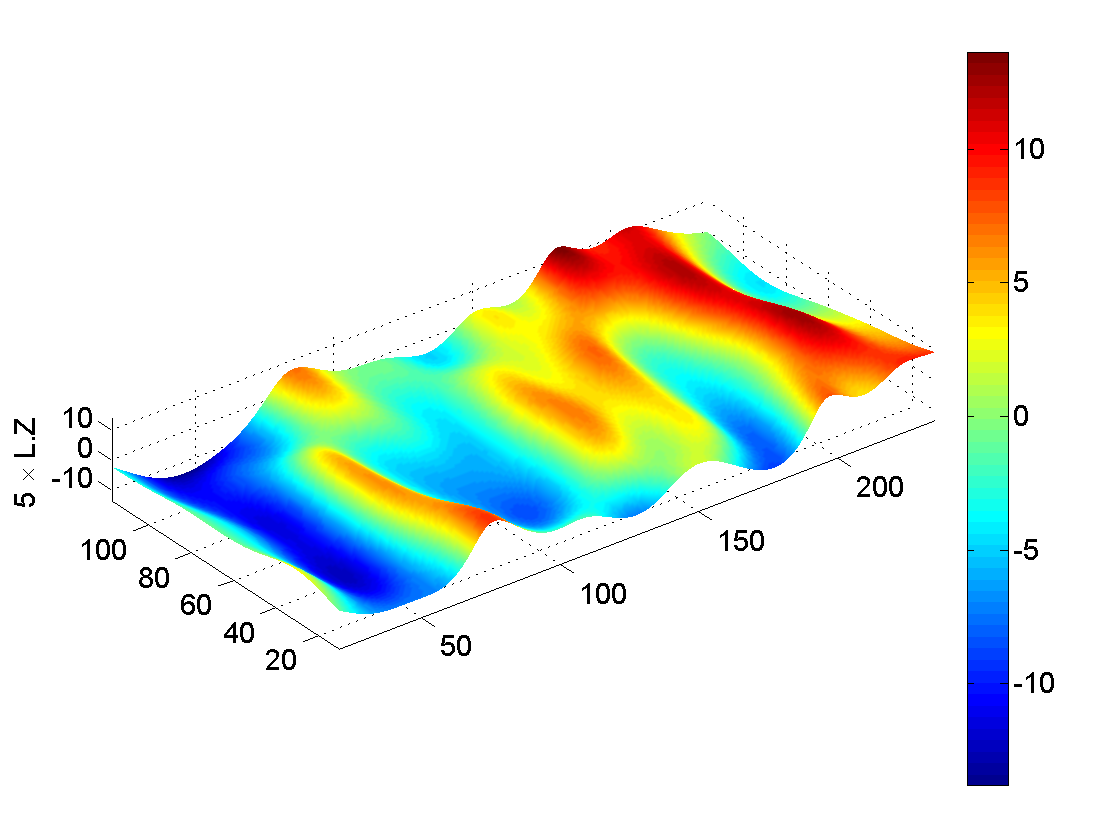
\includegraphics[width=0.7\textwidth]{OneField}
}
\caption{A front-back asymmetric Lagrange field with strong directionality, generated by {\tt ldat2lwav3D}.}
\label{OneField}
\end{figure}
\subsubsection*{Generating a movie}
\addcontentsline{toc}{subsubsection}{\numberline{}Generating a movie}
The option {\tt opt3D.type = 'moviedata'} (or simply {\tt 'movie'}) generates data for a 3D wave movie.
The output from is a structure that can generate wave movie by means of the routine {\tt seamovie}.
%; this is a version of the {\sc Wafo} routine {\tt seamovie} adapted for the dimension standard in {\sc Wafo}L.

We use the options
{\small\begin{verbatim}
   optTime = simoptset('Nt',1001,'dt',0.2,...
                          'Nu',128,'du',10,'Nv',64,'dv',10);
   opt3D = genoptset('type','movie')
\end{verbatim}
}
\noindent
to generate wave movie data
{\small\begin{verbatim}
   [W,X,Y] = spec2ldat3D(SD15,optTime,'lalpha',1.5)
   opt3D = genoptset(opt3D,'start',[20 10])
   Lmovie = ldat2lwav3D(W,X,Y,opt3D)
\end{verbatim}
}
\noindent that, besides producing the movie structure {\tt Lmovie}, plots that last frame of the movie.

The movie is generated and displayed by a command
{\small\begin{verbatim}
   Mv = seamovie(Lmovie,displaytype)
\end{verbatim}
}
\noindent where {\tt displaytype} can take values {\tt 1, 2, 3}. A value {\tt 1} gives a surf-type perspective  movie like field in Figure~\ref{OneField}, a value {\tt 2} gives moving contours at still vater level. {\tt displaytype = 3} give a grayscaled movie. The last frames with the two latter options are shown in Figure~\ref{TwoMovieFrames}.
{\small\begin{verbatim}
   Mv2 = seamovie(Lmovie,2); pause
   Mv3 = seamovie(Lmovie,3); pause
\end{verbatim}
}

\begin{figure}
\centerline{
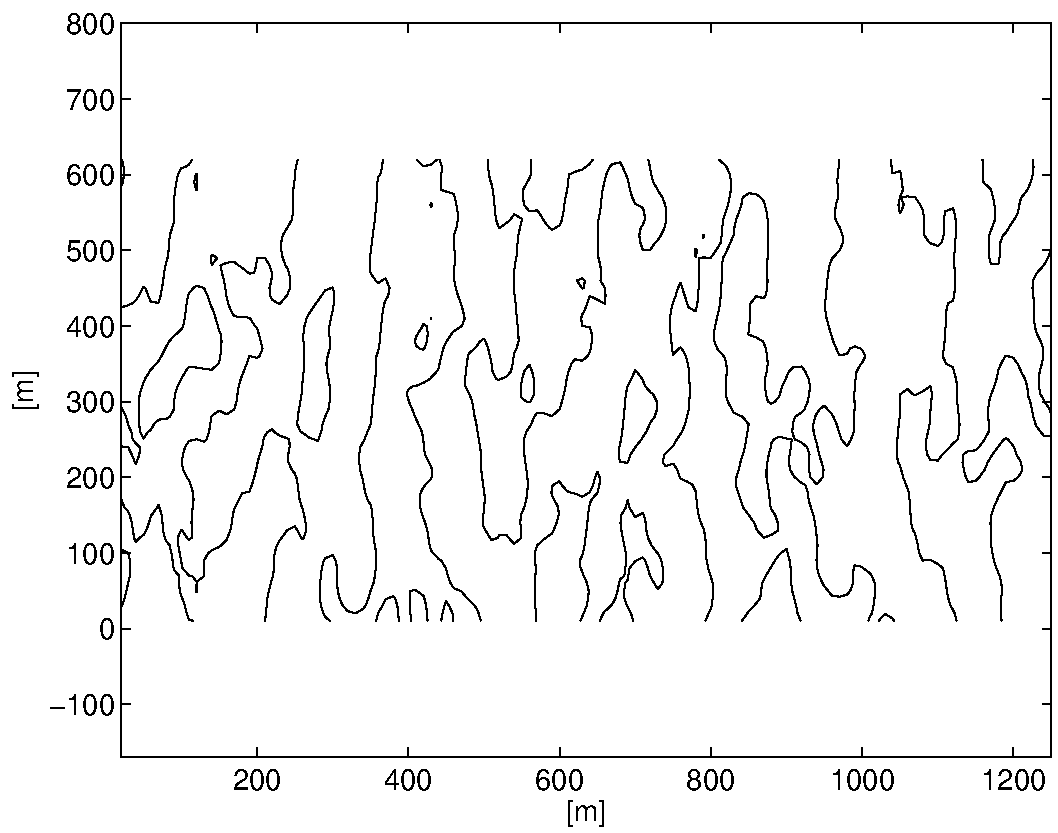
\includegraphics[height=45mm]{Movie2}
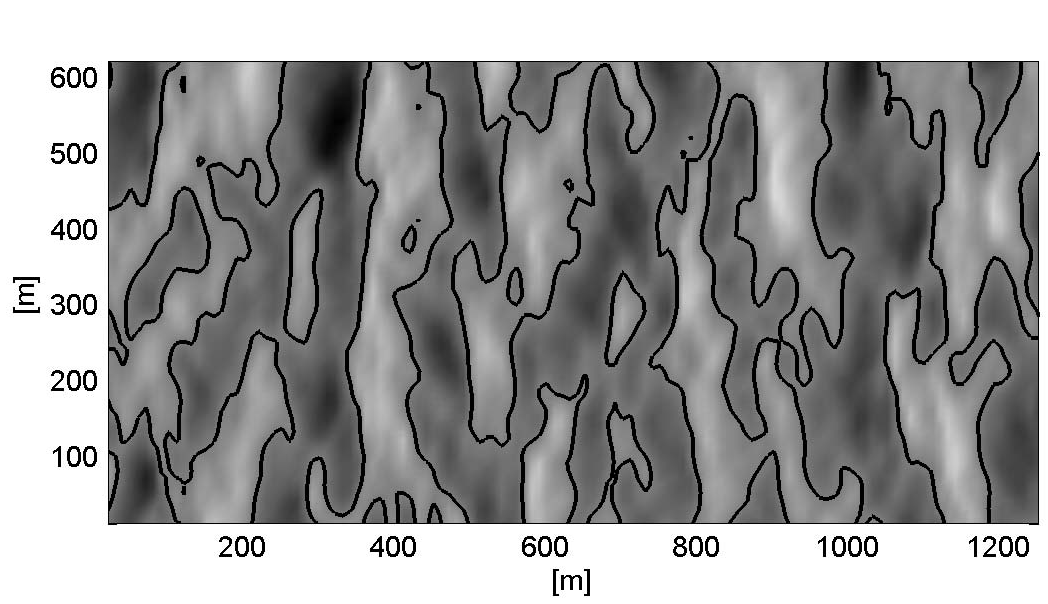
\includegraphics[height=45mm]{Movie3b}
}
\caption{Frames of wave movie; option {\tt displaytype} = 2 (left) and  3 (right).}
\label{TwoMovieFrames}
\end{figure}

Beware that the movie structures are about 10 times bigger than the data structure {\tt Lmovie} that is used to generate the movie.

\subsubsection*{Generating time series}
\addcontentsline{toc}{subsubsection}{\numberline{}Generating time series}
The third type option in {\tt genoptset} is {\tt timeseries}, used to extract pointwise time series wave data obtained at one or more fixed locations. We illustrate how to obtain three time series, observed at three locations along the center line of the area:
{\small\begin{verbatim}
   opt3D=genoptset('type','timeseries','PP',[400 425 450; 300 300 300])

opt3D =

        type: 'timeseries'
          t0: []
          PP: [2x3 double]
       start: [10 10]
         end: []
        rate: 1
    plotflag: 'on'
\end{verbatim}
}

We use the elementary wave data {\tt W,X,Y} from the movie example and generate the three time series, and plot the result in Figure~\ref{Fig-ThreeSeries}:
{\small\begin{verbatim}
   Lseries = ldat2lwav3D(W,X,Y,opt3D,'plotflag','off')
   subplot(311)
   plot(Lseries.t,Lseries.Z{1},'r')
   grid on; hold on
   plot(Lseries.t,Lseries.Z{2},'g')
   plot(Lseries.t,Lseries.Z{3},'b')
\end{verbatim}
}

\begin{figure}[tbh]
\centerline{
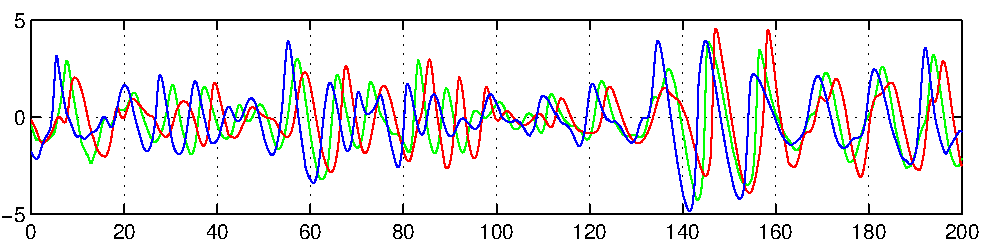
\includegraphics[width=0.8\textwidth]{TreeSeries}
}
\caption{Three wave time series separated 25 meters in wind direction. Blue curve: upwind station, red curve: downwind station.}
\label{Fig-ThreeSeries}
\end{figure}

Figure~\ref{Fig-CCF} shows the cross-correlation function between the upwind and the downwind series, taken at a distance of 50 meters. We use the {\sc Matlab} routine {\tt xcov} in the signal processing toolbox.
{\small\begin{verbatim}
   Rx = xcov(Lseries.Z{1},Lseries.Z{3},200,'biased)
   subplot(211)
   plot((-200:200)/5,Rx,'LineWidth',2,'FontSize',15)
\end{verbatim}
}

\begin{figure}[tbh]
\centerline{
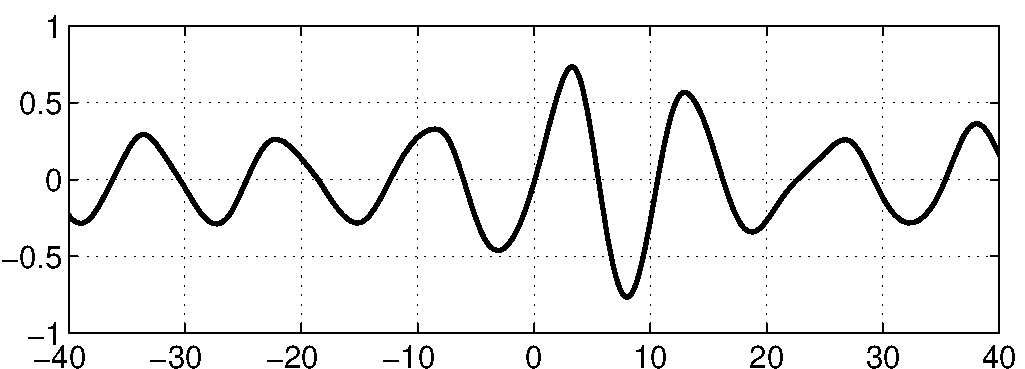
\includegraphics[width=0.6\textwidth]{CCF}
}
\caption{Cross-correlation function between upwind and downwind time series; maximum correlation at time lag 3 seconds, in agreement with ``average wave speed'' of 17 seconds and peak period of 11 seconds.}
\label{Fig-CCF}
\end{figure}

\subsection{Generation of multiple time series from 3D spectrum}
The routine {\tt spec2lseries} generates several time series directly from the directional 3D spectrum without the route via {\tt spec2ldat3D} and {\tt ldat2lwav3D}. The call is
{\small\begin{verbatim}
   L = spec2lseries(Spec3D,PP,options)
\end{verbatim}
}
\noindent
where {\tt PP = [x1 x2 ... xn; y1 y2 ... yn]} defines the coordinates for the observations.  This direct routine will generate the same result and it takes about the same total time as the combined route, but it is much less memory demanding. In particular, the memory requirement is almost independent of the length and number of the time series.  

If you want to compare the two methods, be sure to set {\tt options.iseed} to a suitable integer -- the default value is {\tt shuffle}, i.e. {\tt random} and set {\tt opt3D.start = [0 0]}. Note that  {\tt opt3D.start} is not used in the direct routine; be sure that the observation points are well inside the generated region.

\subsection{Run and export movies}
You might want to export a wave movie for use outside \ML{}, 
for example, publish it on a web-page or send it by e-mail. 
Then you can use the \verb+seamovie+ to save the movie as an avi-file. Just add a a name string, e.g. 'Wave.avi' as a third argument: 
{\small\begin{verbatim}
   Mv1 = seamovie(L,1,'Wave.avi');
\end{verbatim}
}
\noindent
If the current folder already contains a movie {\tt Wave.avi} then a movie with a random name is produced. The extension {\tt .avi} will be automatically added if missing. 

The routine {\tt seamovie} uses the \ML{}-command {\tt movie2avi} which puts restrictions on the \ML{-installation}. It works without extra work, at least, with version 8.5. 
The movie structures are usually large files and the avi-files generated are even larger. 
It is recommended that you edit them with a video editing program and save in some other format, e.g. {\tt mp4}, to facilitate distribution. 

\chapter{2$^{nd}$ order non-linear Lagrange waves}\label{Secondorderwaves}
\section{Euler, Gauss, Lagrange, and Stokes waves}
\subsection{Gauss and 2$^{nd}$ order Stokes interaction}
The Gaussian waves model \eqref{2DGauss} describes the water surface as the sum of statistically independent harmonic components, acting without interaction between distinct frequencies. The 2$^{nd}$ order Stokes model also contains sums of harmonics with frequencies equal to the sums and differences, in simplified form, 
\begin{align}
\text{ 1$^{st}$ order term} &: w_1(t) = m + \sum A_j \cos ( \omega_j t + \theta _j) 
= m +\Re \sum Z_j e^{i \omega_j t}, \label{ww} \\
\text{2$^{nd}$ order term} &: w_2 (t) = 
\Re \sum Z_j Z_k \, H_{jk}^+ \, e^{i(\omega_j + \omega_k) t}  +
\Re \sum Z_j Z_k^* \, H_{jk}^- \, e^{i(\omega_j - \omega_k) t} ,  \label{yy} \\
\text{Total wave} &: w(t)  = w_1(t) + w_2(t). \nonumber
\end{align} 
Here, the complex variables $Z_j$ define both amplitudes and phases 
of the harmonics and $^*$ denotes complex conjugate. The factors $H_{jk}^+$ and  
$H_{jk}^-$ are ``2$^{nd}$ order transfer factors'', and they are quite complicated depth dependent functions of the frequencies $\omega_j$ and the corresponding wave-numbers $\kappa_j$;  \cite{MarthinsenAndWinterstein1992Skewness,Nouguieretal2015,Prevosto1998}. Equations (\ref{ww}-\ref{yy}) give an ``Euler'' description of the water elevation at a fixed location. 

\subsection{Lagrange and 2$^{nd}$ order Stokes interaction}
In the Gauss-Lagrange model the vertical and horizontal displacements are 
correlated Gaussian processes. In the Stokes-Lagrange model, 
also the horizontal processes have an added 2$^{nd}$ order term 
of the same type as \eqref{yy}, but with special transfer factors, \cite{fouqueskrogstadmyrhaug2006,Nouguieretal2015,Prevosto1998}. 
The horizontal components furthermore contain a random drift term, $d_x(t), d_y(t)$, 
constant in time, called the ``Stokes drift''.

 Figure~\ref{FigFilter} illustrates the linear filters, ${\cal L}_{zw}^1, {\cal L}_{zw}^1$, between the generating elements $\{Z_j\}$ and the Gaussian components, and the quadratic filters from 
$w_1, x_1$ to $w_2, x_2$.  

\begin{figure}
\centerline{
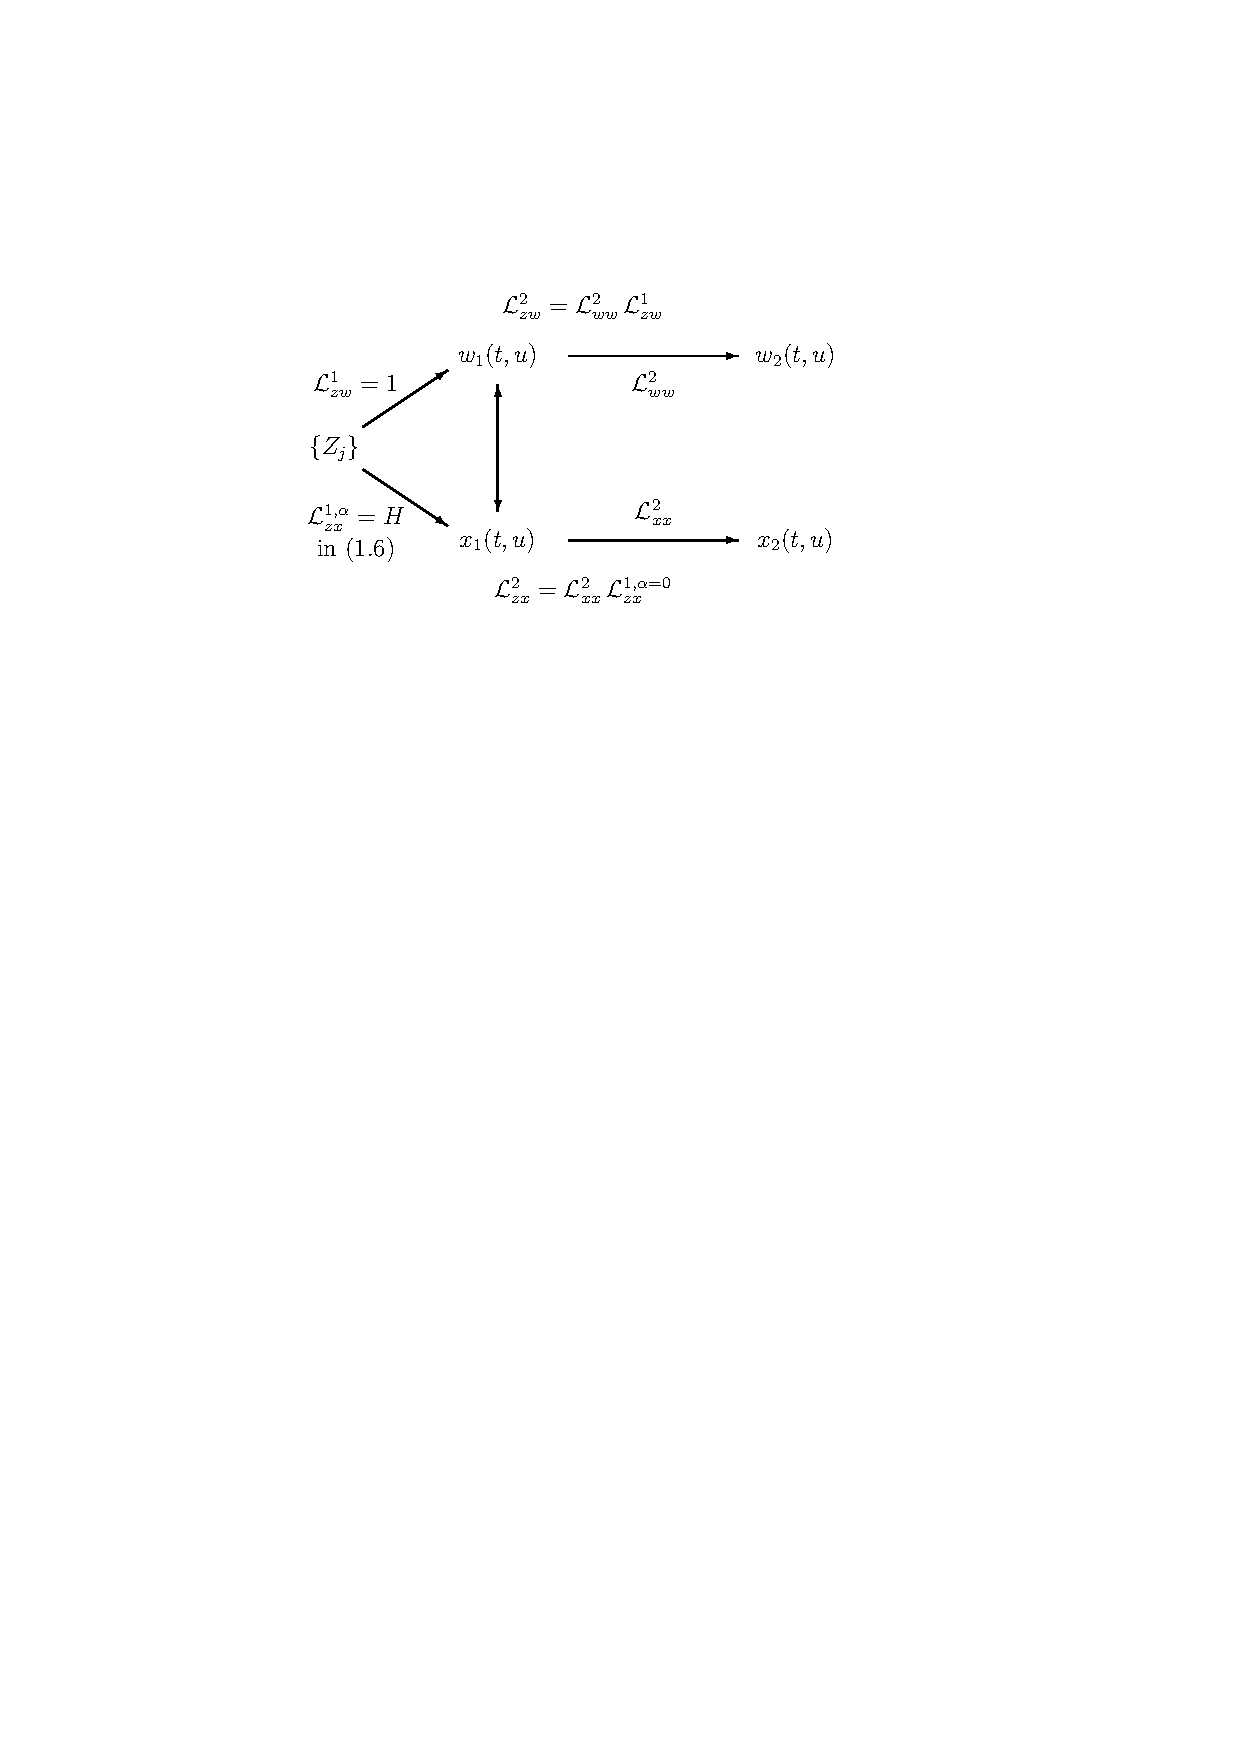
\includegraphics[width=100mm]{Picture}
}
\caption{Schematic view of the generation of wave components from $\{Z_j\}$  in \eqref{ww}.}
\label{FigFilter}
\end{figure}

\subsection{{\sc Wafo} and {\sc WafoL} routines for \fo and \so order waves}
%1$^{st}$ and 2$^{nd}$ order waves}
The {\sc Wafo} toolbox contains the routine {\tt spec2nlsdat} for simulation of 
2D Stokes-Euler waves. It is an extension of the (Euler) routine {\tt spec2sdat} whose {\sc Wafo}L version is {\tt spec2ldat}. The {\sc Wafo} routine {\tt seasim} has the {\sc Wafo}L extension {\tt spec2ldat3D}; both generate 3D waves. 
 
The {\sc Wafo}L routines  {\tt spec2ldat3DM} and {\tt spec2ldat3DP} are 3D Stokes-Lagrange companions to  {\tt spec2nlsdat}. They can be used to produce the components for 2D and 3D Stokes-Lagrange waves, including the Stokes drift. 
{\tt spec2ldat3DM} is a (M)odification and extension 
of the {\sc Wafo}L routine {\tt spec2ldat3D} and {\tt spec2ldat3DP} is a version arranged for (P)arallel processing with the  Parallel Computing Toolbox in \ML{}. 

Table~\ref{TabSpec2routines} lists the capabilities of different {\sc Wafo} and {\sc Wafo}L routines to simulate the components of linear and non-linear waves, based on the Gaussian generator $\{Z_j\}$.  

\begin{table}[tbh]
\centerline{
\begin{tabular}{|l|c|c|c|c|c|c|c|c|} \hline &
\multicolumn{1}{c|}{
\begin{sideways}{\parbox[b]{2cm}{\raggedright\textbf{Gauss-Euler}}}\end{sideways}} 
&\multicolumn{1}{c|}{
\begin{sideways}{\parbox[b]{22mm}{\raggedright\textbf{Gauss-Euler}}}\end{sideways}} 
& \multicolumn{1}{c|}{
\begin{sideways}{\parbox[b]{22mm}{\raggedright\textbf{Gauss-Lagrange}}}\end{sideways}} 
& \multicolumn{1}{c|}{
\begin{sideways}{\parbox[b]{22mm}{\raggedright\textbf{Gauss-Lagrange}}}\end{sideways}} 
& \multicolumn{1}{c|}{
\begin{sideways}{\parbox[b]{22mm}{\raggedright\textbf{Stokes-Euler}}}\end{sideways}} 
& \multicolumn{1}{c|}{
\begin{sideways}{\parbox[b]{22mm}{\raggedright\textbf{Stokes- Euler}}}\end{sideways}} 
& \multicolumn{1}{c|}{
\begin{sideways}{\parbox[b]{22mm}{\raggedright\textbf{Stokes- Lagrange}}}\end{sideways}} 
& \multicolumn{1}{c|}{
\begin{sideways}{\parbox[b]{22mm}{\raggedright\textbf{Stokes- Lagrange}}}\end{sideways}} \\
& {\bf 2D} & {\bf 3D} & {\bf 2D} & {\bf 3D}  & {\bf 2D} & {\bf 3D} 
& {\bf 2D} & {\bf 3D} \\ \hline  
{\sc\bf Wafo} &&&&&&&& \\
{\tt spec2sdat} & \bplus & \bminus & \bminus & \bminus & \bminus & \bminus & \bminus & \bminus \\
{\tt seasim} & \bplus & \bplus & \bminus & \bminus & \bminus & \bminus & \bminus & 
\bminus \\
{\tt spec2nlsdat} & \bplus & \bminus & \bminus & \bminus & \bplus & \bminus & \bminus & \bminus \\  \hline
{\bf {\sc\bf Wafo}L} &&&&&&&& \\ 
{\tt spec2ldat} & (\bplus) & \bminus & \bplus & \bminus & \bminus & \bminus & \bminus & \bminus \\
{\tt spec2ldat3D} & (\bplus) & (\bplus) & \bplus & \bplus & \bminus & \bminus & \bminus & \bminus \\  \hdashline
{\tt spec2ldat3DM} & (\bplus) & (\bplus) & \bplus & \bplus & (\bplus) & (\bplus) & \bplus & \bplus \\
{\tt spec2ldat3DP} & (\bplus) & (\bplus) & \bplus & \bplus & (\bplus) & (\bplus) & \bplus & \bplus \\ \hline  
\end{tabular}}
\caption{Spectral based simulation routines in {\sc Wafo} and {\sc Wafo}{\sc L}}
\label{TabSpec2routines}
\end{table}

\subsection{A comment on terminology}
In the table we have used the terms ``Euler'' and ``Lagrange'' in an un-orthodox way. In hydrodynamics they denote two equivalent ways to define the physics of water waves, 
where an Euler description is focused on the velocity field at each fixed coordinate, 
while the Lagrange description integrates the velocity fields to get the trajectories of
 individual particles. The {\sc Wafo} routines are basically stochastic Euler routines, 
dealing only with the statistical properties of the vertical variation of the free surface,  in the simplest form  as a Gaussian process.

In the Lagrange wave model, as described in this tutorial, and in most publications on the topic, one simply borrows the Gaussian process from the Euler description and uses it as a Lagrange description of particle movements, with vertical and horizontal proceses related by a hydrodynamicaly motivated linear filter equation.  A quadratic filter then brings the Gauss model into a Stokes model. The {\sc Wafo}L routines {\tt spec2ldat, spec2ldat3D, spec2ldat3DM/P}  generate such 1$^{st}$ and 2$^{nd}$ order Lagrange data {\tt ldat}. 

The routines {\tt ldat2lwav} and {\tt ldat2lwav3D} bring Lagrange data (of any order) into an easily observable Euler model. In fact, empirical Lagrange data on particle trajectories are rare, compared to the abundance of Euler data.  Thus, our Lagrange routines not only simulate trajectories, but, with some extra effort, also the Euler observables.  This explains the {\tt (+)} notations in 
Table~\ref{TabSpec2routines}.


\section{Generating 1$^{st}$ order processes} % with {\tt spec2ldat3DM}}
\subsection{Introduction to the routines}
The routine {\tt spec2ldat3DM} generates 1$^{st}$ and 2$^{nd}$ order 
ingredients to a 3D Lagrange field, with a call similar to that of {\tt spec2ldat3D} but with an extra parameter, {\tt order}:  
{\small\begin{verbatim}
   [W,X,Y] = spec2ldat3DM(Spec,order,options); % order = 1  
   [W,X,Y,W2,X2,Y2] = spec2ldat3DM(Spec,order,options); % order = 2
\end{verbatim}
}

The input directional spectrum is defined by a one-sided spectrum structure with the direction dependence specified by a separate 
field.\footnote{The {\sc Wafo}L  version~1.1.1 of {\tt spec2ldat3DM} does not allow input of a directional spectrum with frequency dependent spreading. 
Thus, only frequency independent spreading is possible at present.} 
Set up the spectrum information and simulation options as follows: 
{\small\begin{verbatim}
   S = jonswap;
   D = spreading(linspace(-pi,pi,91),'cos2s',0,10,S.w,0);  % Here, the last
        % parameter is set to 0  to give frequency independent spreading
   S.h = 40;
   S.D = D; % This extra field carries the spreading information 
   Sdir = mkdspec(S,D);     
   plotspec(Sdir)
   option = simoptset('Nt',1001,'dt',0.2,'Nu',300,'du',1,'Nv',100,'dv',1);
\end{verbatim}
}
\noindent
Note that the spectrum structure {\tt S} with the extra field {\tt S.D = D} carries the same information as the directional spectrum {\tt Sdir}. They are used as input in 
{\tt spec2ldat3D} and in {\tt spec2ldat3DM, spec2ldat3DP}, respectively. 

\begin{SCfigure}[1][tbh]
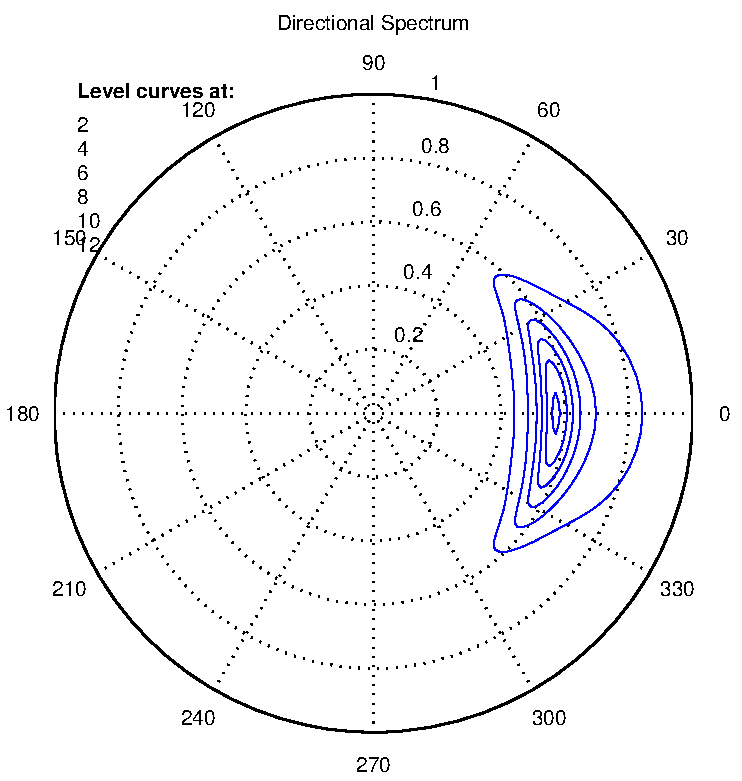
\includegraphics[width=0.4\textwidth]{Fig31}
\caption{Directional spectrum with frequency independent spreading; cf.\ Figure~\ref{Dspec_dir}.}
\label{Fig31}
\end{SCfigure}
\subsection{A comparison of execution times for 1$^{st}$ order models}
We start by comparing the execution times obtained with  {\tt spec2ldat3D}, {\tt spec2ldat3DM}, and {\tt spec2ldat3DP} with parallel computing activated. The first routine uses a two-dimensional FFT over space, looping over time, the two others use a one-dimensional FFT over time, looping over x- and y-space directions.  

First generate the elements by the different routines and compare the distributions; they should be equal, but small differences must be expected.
{\small \begin{verbatim}
   [W1,X1,Y1] = spec2ldat3D(Sdir, option); 
   [W2,X2,Y2] = spec2ldat3DM(S,1, option); 
   % matlabpool local 4  % Run if PCT is available
   %[W3,X3,Y3] = spec2ldat3DP(S,1, option); 

   figure(2), clf
   subplot(221)
   qqplot(W1.Z(:),W2.Z(:)); grid on
   xlabel('W1.Z quantiles')
   ylabel('W2.Z quantiles')
   subplot(222)
   plotnorm(W1.Z(:))
\end{verbatim}
}

\begin{figure}[tbh]
\centerline{%
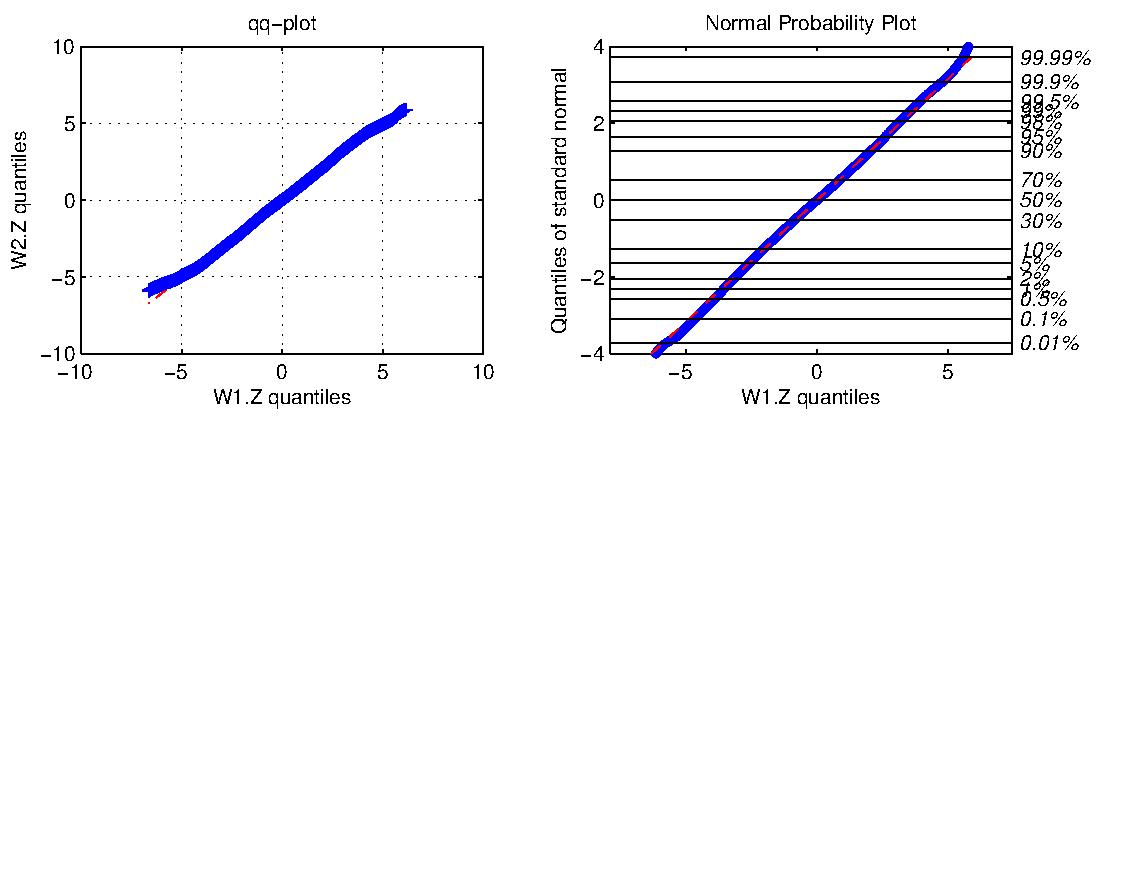
\includegraphics[width=0.8\textwidth]{Fig32}
}
\caption{Right: normal plot of {\tt W1.Z} generated by {\tt spec2ldat3D}. Left: a {\tt qqplot} comparison 
with {\tt W2.Z} generated by {\tt spec2ldat3DM}.} 
\label{Fig32}
\end{figure}
We have run each of the commands 100 times to get the execution time and total standard deviation for each of the components, {\tt std(W.Z(:))}, etc., for each simulation,  and then calculated the average and standard deviations. 
\begin{table}
\centerline{
\begin{tabular}{l|ccc}
Routine & {\tt spec2ldat3D}& {\tt spec2ldat3DM}& {\tt spec2ldat3DP} \\ \hline
Relative exec time & 1 (2.3\%) &  1.32 (0.9 \%)& 1.05 (1.5\%) \\
Mean std {\tt W.Z} & 1.75 (0.26) & 1.72 (0.19)& 1.70 (0.17) \\
Mean std {\tt X.Z} &4.36 (0.89) & 4.26 (0.64) & 4.20 (0.57) \\
Mean std {\tt Y.Z} &1.53  (0.32) & 1.46 (0.19) & 1.46 (0.18) \\ \hline
\end{tabular}
} 
\caption{Relative execution times and obtained average standard deviations for the three components, {\tt W.Z}, {\tt X.Z}, and {\tt Y.Z}, simulated 100 times; numbers in parenthesis are the observed relative standard deviation, and standard deviations of the measured quantities, respectively. The absolute execution time is about 35 seconds per simulation with {\tt spec2ldat3D}. }
\label{TabExTime1}
\end{table}

We can draw two conclusions from the results in  Table~\ref{TabExTime1}. 
As seen, the execution time is about the same for {\tt spec2ldat3D}, 
with two-dimensional FFT,  and {spec2ldat3DP}, with one-dimensional FFT 
and parallelization, while the non-parallelized version takes 32\% more time. 
One possible  reason that {\tt spec2ldat3D} can compete with {\tt spec2ldat3DP} is that in the first routine, the space grid internally  is optimized for {\tt fft2}, stepping only in time, while in the second routine the parallelization is used in the {\tt u}-variable, stepping over the {\tt v}-variable, to perform a less time-consuming {\tt fft} in the time-variable.  As a consequence, the relative speed of the two routines will vary with the dimensions in time and space. 

One can also note that the observed standard deviation of {\tt W.Z} is slightly less than 
{\tt 1.75 = Hs/4} for two of the routines. This is an effect of the relative sparsity of the spectral density discretization, which is automatic from the time parameters, and leads to a small loss in energy.  This phenomenon can also occur for {\tt spec2ldat3D }. 

Regardless of how the {\tt ldat}-structures {\tt W,X,Y} are generated, they can be used as in Chapter~\ref{3DLagrangeWaves} by 
{\tt ldat2lwav} and {\tt ldat2lwav3D} to generate a Lagrange wave or wave field. 

The motivation for the routines {\tt spec2ldat3DM} and {\tt spec2ldat3DP} is that they can generate 2$^{nd}$ order corrections both in the vertical component and in the horizontal components; then the parallelization is very effective. 

\subsection{Some differences between the two methods for 2D waves} 
The routines {\tt spec2ldat3DM/P} can take a non-directional spectrum structure as spectral argument and generate the vertical, {\tt W.Z}, and horizontal, {\tt X.Z}, components for a 2D Lagrange wave. One should expect the result would be the same as that produced by {\tt spec2ldat}, but there are some differences. 
\begin{itemize}
\item {\tt spec2ldat3DM/P} use the number of frequencies in the spectrum to decide on the number of time points to be generated. The spectrum is interpolated to reach the approximate time span as specified by {\tt W.t(end) = (opt.Nt-1) * opt.dt}.
\item {\tt spec2ldat} change an odd value of {\tt Nt} to the nearest greater even value; (similar with {\tt Nu} if {\tt ffttype = 'fftspace'}). 
\end{itemize}

We issue the following commands in order to simulate {\tt W, X} over 250 seconds with sampling rate 2 Hz, i.e. we set {\tt Nu=501, dt=0.5}, and ask for the resulting {\tt W, Wm}: 
{\small\begin{verbatim}
   S = jonswap;   opt = simoptset('Nt',501,'dt',0.5,'Nu',1001,'du',1);
   [W,X] = spec2ldat(S,opt);   [Wm,Xm] = spec2ldat3DM(S,1,opt);

   W = 

                 Z: [1001x502 double]     
                 u: [1001x1 double]
                 t: [1x502 double]
              note: [1x41 char]
               std: 1.6650
        meanperiod: 8.4879
    meanwavelength: 112.4406

   Wm = 

       Z: [1001x516 double]
       u: [1001x1 double]
       t: [516x1 double]
\end{verbatim}}

\noindent
We note the change in the number of time steps, while the number of space steps is unchanged. The generated time spans are {\tt W.t(end) = 250.5000} and {\tt Wm.t(end) = 250.0145}. Thus, neither routine gives the exact time span, {\tt 250}, that we expected! 

\subsection{Using the data from {\tt spec2ldat3DM/P}}
The {\tt ldat} produced by {\tt spec2ldat3DM/P} have the same structure as that produced 
by {\tt spec2ldat3D} and it can be used as described in Chapter~\ref{3DLagrangeWaves}. However, since {\tt spec2ldat3D} usually is the faster routine one may prefer that for 1$^{st}$ order simulation.

\section{Generating 2$^{nd}$ order 2D waves}\label{s:22waves}
We now turn to the main theme of this chapter, generation of 2$^{nd}$ order Lagrange waves. The {\sc Wafo} toolbox contains the routine {\tt spec2nlsdat} for generation of 2$^{nd}$ order 2D Stokes-Euler waves.  With {\tt spec2ldat3DM/P} one can generate both 2D and 3D Stokes-Lagrange waves, and we start with the 2D case. 

\subsection{2D Stokes time waves with {\tt spec2nlsdat}}\label{ss:Stokesnlsdat}
As listed in Table~\ref{TabSpec2routines} there are two routines that generate 2D Stokes waves, the {\sc Wafo} routine {\tt spec2nlldat}, which directly generate a Stokes time wave at a single point, and the more general {\sc Wafo}L routines {\tt spec2ldat3DM/P}, which give the Lagrange components, which combined with {\tt ldat2lwav}  give the time wave.

We use the  {\sc Jonswap} spectrum without spreading, and set the depth to {\tt S.h=20}. 
{\small\begin{verbatim}
   S = jonswap; S.h = 20;   np = 250; dt = 0.2;
   [xs2 xs1] = spec2nlsdat(S,np,dt);
   figure(1); clf
   waveplot(xs1,'r',xs2,'b',1,1)
\end{verbatim}}

\begin{SCfigure}[0.8][b]
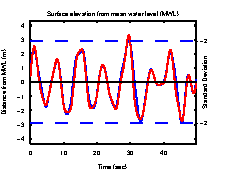
\includegraphics[width=0.55\textwidth]{Nls_4}
\caption{A {\tt waveplot} of  linear (blue) and non-linear (red) time wave generated 
by {\tt spec2nlsdat}.}
\label{Fig:nls}
\end{SCfigure}

\noindent
The result is the Gaussian time wave {\tt xs1}, a two-column array with time in the first and the vertical 
height in the second column, and the 2$^{nd}$ order Stokes wave 
{\tt xs2}.  We use {\tt waveplot} to show the result in 
Figure~\ref{Fig:nls}; see {\tt help waveplot}.

\subsection{2D Stokes waves with {\tt spec2ldat3DM/P} and {ldat2lwav}}
As shown in Chapter~\ref{3DLagrangeWaves} the routine {\tt ldat2lwav3D} 
can give all kinds of observable wave data from the Lagrange 
components {\tt W,X,Y}. The option {\tt opt3D.type = 'timeseries'} will lead to one or more 
timeseries, of the same type as the {\tt xs1,xs2} waves produced by {\tt spec2nlsdat}. 
In this section we want only 2D waves and use a uni-directional spectrum and set {\tt opt.Nv = 1}. 
Note the result,  that the Stokes drift in {\tt X2} is negative directed in the main wave direction. 
{\small\begin{verbatim}
   S = jonswap; S.h = 20;
   opt = simoptset('Nt',250,'dt',0.2,'Nu',1001,'du',1,'Nv',1);
   [W,X,~,W2,X2,~] = spec2ldat3DM(S,2,opt);
   X2.drift(end,end) 
\end{verbatim}
}

\subsubsection*{Time waves}
We now construct two sets of 2$^{nd}$ order components, one with Stokes drift and one without, and 
generate the timeseries observed at location {\tt 250} and plot the three series:
{\small\begin{verbatim}
   Wtot2 = W; Wtot2.Z = W.Z + W2.Z;
   Wtot2d = Wtot2;  % No Stokes drift in the vertical direction ! 
   Xtot2 = X; Xtot2.Z = X.Z + X2.Z;
   Xtot2d = X; Xtot2d.Z = X.Z + X2.Z + X2.drift;
   [L,L0] = ldat2lwav(W,X,'time',250,1,0);
   [L2,L20] = ldat2lwav(Wtot2,Xtot2,'time',250,1,0);
   [L2d,L20d] = ldat2lwav(Wtot2d,Xtot2d,'time',250,1,0);

   plot(L0.t,L0.Z,'b'); hold on, grid on;
   plot(L20.t,L20.Z,'r-.')
   plot(L20d.t,L20d.Z,'r'); hold off
\end{verbatim}
}

Figure~\ref{Fig:nlsStokes} shows the effect of the Stokes drift, shifting the peaks in time. Observe that the 
shapes of shifted and non-shifted waves are different, since they have different reference coordinates, i.e. 
they have different origin in space. 
\begin{SCfigure}[0.8][b]
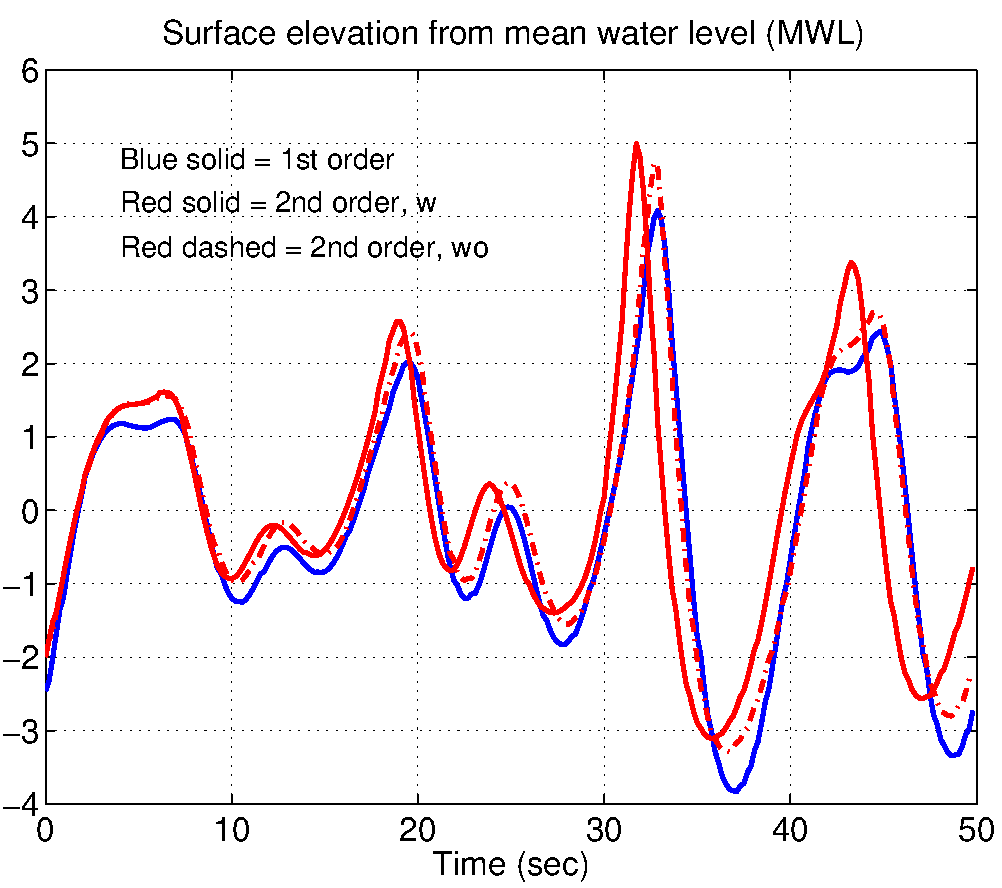
\includegraphics[width=0.46\textwidth]{Nls_6}
\caption{Time waves:  1$^{st}$ order (blue) and 2$^{nd}$ order with (red, solid) and without (red, dashed) Stokes drift.}
\label{Fig:nlsStokes}
\end{SCfigure}

\subsubsection*{Space waves}
We use the component processes to generate space waves by means of {\tt ldat2lwav}, but first we increase the time interval: 
{\small\begin{verbatim}
   S = jonswap; S.h = 20;
   opt = simoptset('Nt',1000,'dt',0.2,'Nu',1001,'du',1,'Nv',1);
   [W,X,~,W2,X2,~] = spec2ldat3DM(S,2,opt); 
\end{verbatim}
}

We generate the space waves at three timepoints, {\tt 50, 100, 150} to see the effect of the Stokes in relation to the 2$^{nd}$ order effect, and plot the results in Figure~\ref{Fig:Nls_space}, (for plotting commands, see {\tt WafoLCh3.m}). 

{\small\begin{verbatim}
   Wtot2 = W; Wtot2.Z = W.Z + W2.Z;
   Xtot2d = X; Xtot2d.Z = X.Z + X2.Z + X2.drift;
   
   [L50,L050] = ldat2lwav(W,X,'space',50,1,0);
   [L2d50,L20d50] = ldat2lwav(Wtot2d,Xtot2d,'space',50,1,0);
   [L100,L0100] = ldat2lwav(W,X,'space',100,1,0);
   [L2d100,L20d100] = ldat2lwav(Wtot2d,Xtot2d,'space',100,1,0);
   [L150,L0150] = ldat2lwav(W,X,'space',150,1,0);
   [L2d150,L20d150] = ldat2lwav(Wtot2d,Xtot2d,'space',150,1,0);
\end{verbatim}
}

\begin{SCfigure}[0.8][tbh]
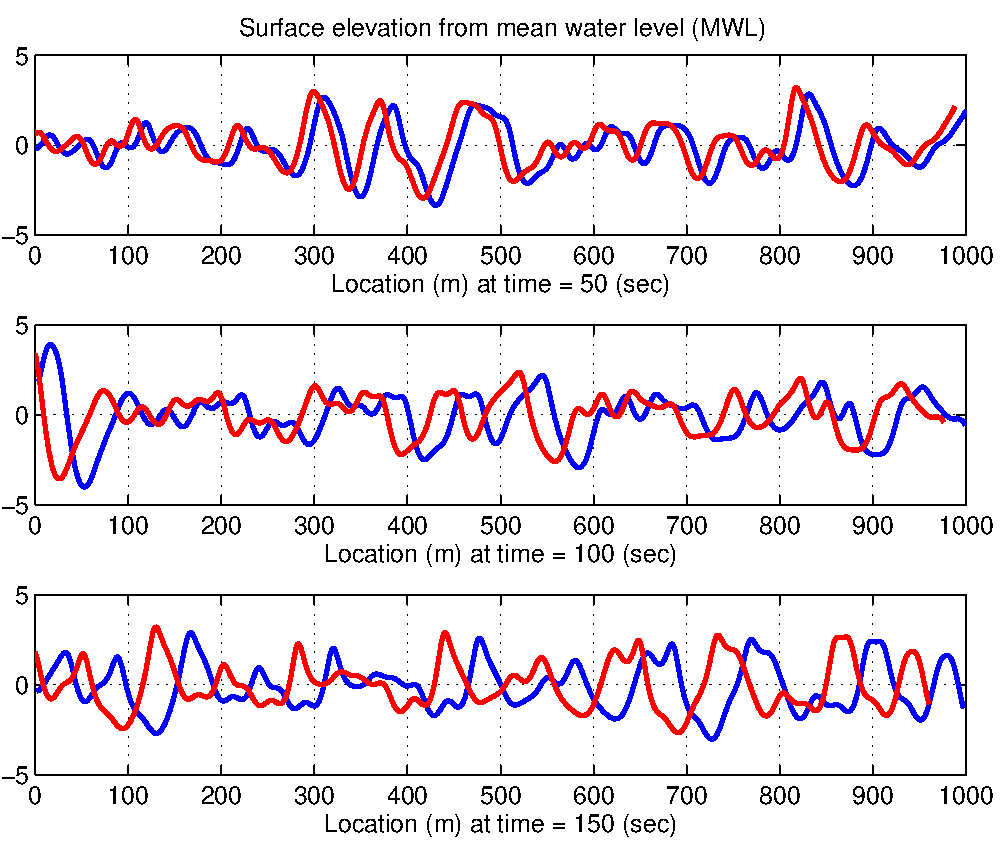
\includegraphics[width=0.5\textwidth]{Nls_space}
\caption{Space waves: 1$^{st}$ order (blue) and 2$^{nd}$ order with Stokes drift (red) at three different time points. Waves move from right to left.}
\label{Fig:Nls_space}
\end{SCfigure}   

\subsection{Wave asymmetry in 2$^{nd}$ order waves}\label{ss:frontbacksecondorder}
The {\sc Wafo} routine {\tt spec2nlsdat} generates 2$^{nd}$ order time waves with typical crest-trough asymmetry, and we saw one example in Section~\ref{ss:Stokesnlsdat}.
 
To generate front-back asymmetric waves we need the Lagrange technique in {\sc Wafo}L, as was described in Sections~\ref{ss:GaussLagrange} and \ref{ss:frontbackasymmetry}. The degree of asymmetry is determined by the parameter $\alpha$, which enters into the transfer function 
${\cal L}_{zx}^{1,\alpha} = H$ in Figure~\ref{FigFilter}. As illustrated in that figure, the $\alpha$  affects only the 1$^{st}$ order and not the 2$^{nd}$ order $X$-component; of course also the $Y$-component is affected in an analogous way. 

We illustrate the effect by simulating the components,
{\small\begin{verbatim}
   [W,X,~,W2,X2,~] = spec2ldat3DM(S,2,opt,'Nt',250,'lalpha',1.5);
\end{verbatim}
}
\noindent
and repeating the commands for the time waves in Figure~\ref{Fig:nlsStokes} to get 
Figure~\ref{Fig:nls_asym}. 
\begin{figure}
\centerline{
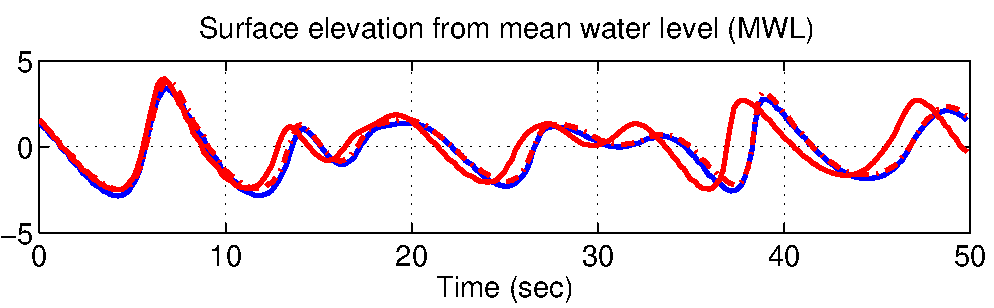
\includegraphics[width=0.7\textwidth]{Nls_asym}
}
\caption{Front-back asymmetric time wave with 2$^{nd}$ order components.}
\label{Fig:nls_asym}
\end{figure}

\section{Generating 2$^{nd}$ order 3D waves}\label{s:23waves} 
 To simulate 2$^{nd}$ order 3D Lagrange waves with {\tt spec2ldat3DM/P} we need a directional spectrum specified by a spectral density structure {\tt S} with a direction field {\tt .D}. We also set a preliminary options structure, make a simulation and take a look at the drift in the main wave direction:
{\small\begin{verbatim}
   S = jonswap; S.h=20;
   D = spreading(linspace(-pi,pi,51),'cos2s',0,15,S.w,0);
   S.D = D;
   opt=simoptset('Nt',250,'dt',0.2,'Nu',250,'du',1,'Nv',50,'dv',1);
   [W,X,W,W2,X2,Y2] = spec2ldat3DM(S,2,opt);
   surf(X2.drift(1:2:end,1:2:end,end)) % To see the drift magnitude
\end{verbatim}
}
\noindent
We see in Figure~\ref{Fig:finalsdrift} that in this simulation the maximal extension of the Stokes drift in the $x$-direction at the end of the time interval is almost 20 meters. This means that if we want to make a movie of the field over a certain region we have to extend the reference region with at least this amount to be sure to capture the variation over the whole region of interest. The drift in the $y$-direction is smaller and less than $\pm 5$ meters.
\begin{SCfigure}[0.8][tbh]
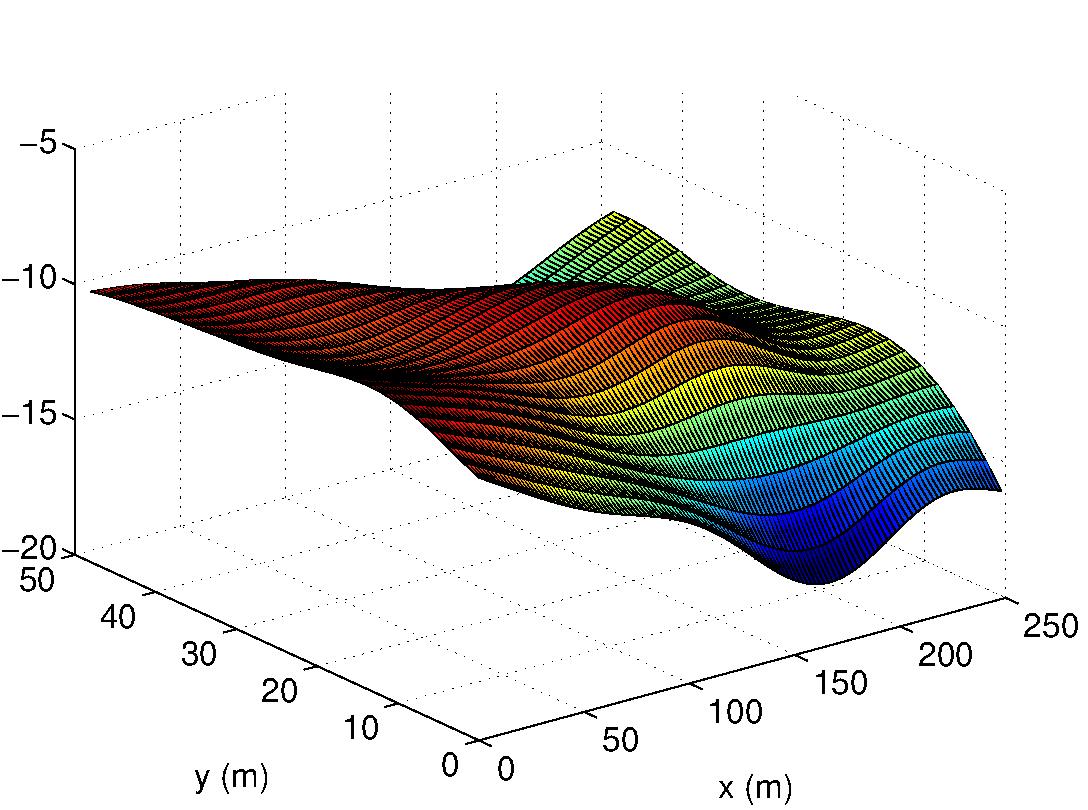
\includegraphics[width=0.6\textwidth]{finalsdrift}
\caption{Stokes drift at the end of the observation interval}
\label{Fig:finalsdrift}
\end{SCfigure}

To be on the safe side, we decide to extend the reference region by 100 meters at the far end, by 10 meters at the near end, and by 15 meters both sideways. Thus, to simulate a 50 seconds wave movie over a region 250 x 100 meters we choose {\tt opt.Nu=360, opt.du=1} and {\tt opt.Nv=130,opt.dv=1}.

Note that, if the reference region is defined too small, a warning is issued, and strange patterns can appear 
at the borders of the simulated region. 
Then one has to extend the reference region to the expense of increased simulation time. 

{\small\begin{verbatim}
   opt=simoptset('Nt',250,'dt',0.2,'Nu',360,'du',1,'Nv',130,'dv',1);
   [W,X,Y,W2,X2,Y2] = spec2ldat3DM(S,2,opt);
   Wtot2 = W; Wtot2.Z = W.Z + W2.Z;
   Xtot2d = X; Xtot2d.Z = X.Z + X2.Z + X2.drift;
   Ytot2d = Y; Ytot2d.Z = Y.Z + Y2.Z + Y2.drift;
   opt3D = genoptset('start',[10 15],'end',[260 115]);
   figure(1);   L=ldat2lwav3D(Wtot2,Xtot2d,Ytot2d,opt3D);
   figure(2);   Mv=seamovie(L,1);
\end{verbatim}
}

Figure~\ref{Fig:finalframes} shows the last wave views in {\tt L} and in {\tt Mv} with different vertical scaling. 
The right hand view has the correct vertical and horizontal scaling while the left hand view exaggerates 
the vertical variation.

For comparison, we can generate front-back asymmetric waves by replacing 
{\tt opt} by, e.g., 
{\small\begin{verbatim}
   optasym = simoptset(opt,'alpha',1.5);
\end{verbatim}}
\noindent and repeating the simulation. Figure~\ref{Fig:finalframes2} shows the result. 


\begin{figure}[t]
\centerline{
\begin{minipage}{\textwidth}
\raisebox{-0.5\height}{\includegraphics[height=50mm]{LastFrameL}}
\hspace{5mm}
\raisebox{-0.5\height}{\includegraphics[height=25mm]{LastFrameM}}
\end{minipage}}
\caption{Last wave views from {\tt ldat2lwav3D} and {\tt seamovie}; symmetric waves.}
\label{Fig:finalframes}
\end{figure}

\begin{figure}[b]
\centerline{
\begin{minipage}{\textwidth}
\raisebox{-0.5\height}{\includegraphics[height=50mm]{LastFrameL2}}
\hspace{5mm}
\raisebox{-0.5\height}{\includegraphics[height=25mm]{LastFrameM2}}
\end{minipage}}
\caption{Last wave views from {\tt ldat2lwav3D} and {\tt seamovie}; asymmetric waves.}
\label{Fig:finalframes2}
\end{figure}

%\subsection{Final comments}
%The Lagrange model reproduces many geometrical properties of ocean waves. 
%Further studies are needed to compare the 2$^{nd}$ and 1$^{st}$ order 
%Lagrange waves with empirical data, with regards to asymmetry, 
%horseshoe like patterns, etc.; 
%\cite{Lindgren2015Waveenergy,Lindgren2015Horseshoe,Nouguieretal2014}.
 
\appendix
\chapter{Commands for the examples}
The command files {\tt WafoLChx.m} contain the code for the examples in the tutorial. Some of the examples take some time and generate big data arrays. You may need to reduce the size of the problems, for example by using a smaller {\tt Nsim} or reduce the dimension.  
Figure titles and other editing are often not included.

The time to run {\tt WafoLCh1} in Windows 10 with Matlab 2017a on an Intel Core i7-7700, 3.60GHz, 32GB RAM, is about 20 minutes, the time for {\tt WafoLCh2} is less than 30 seconds, and that for 
{\tt WafoLCh3} is about 13 minutes. 

The ``pause-state'' is set to {\tt off} in the scripts. Set if to {\tt on} if you want to pause between tasks.
 
\section{{\tt WafoLCh1}, Commands for Chapter 1}
{\small\begin{verbatim}
% Script with commands for WafoL tutorial, Chapter 1

pstate = pause('off');
TSTART = cputime;
disp(' Chapter 1: 2D Lagrange waves')

disp(' Section 1.1.2')
% Figure: Lagrange time wave, example of asymmetry
   S = jonswap; S.h = 20;
   opt = simoptset('dt',1);
   [w,x] = spec2ldat(S,opt,'lalpha',1);
   [L,L0] = ldat2lwav(w,x,'time',[],10);
   subplot(211)
   plot(L.t,L.Z); hold on 
   plot(L0.t,L0.Z,'r')
   axis([0 40 -6 6]); hold off
   pause
   
disp(' Section 1.2.2')
   % Figure: Lagrange space wave, direct plot
   S = jonswap(1.5); S.h = 8;
   opt = simoptset('Nt',256,'dt',0.125,'Nu',...
      256*8,'du',0.25,'iseed',123791);
   [w,x] = spec2ldat(S,opt,'iseed','shuffle')
   subplot(211)
   plot(x.u+x.Z(:,128),w.Z(:,128))
   axis([0 500 -10 10])
   pause
 
disp(' Section 1.2.3')
   % Figure: Lagrange space wave from [L,L0]
   [L,L0] = ldat2lwav(w,x,'space',16)
   subplot(212)
   plot(L.u,L.Z,L0.u,L0.Z,'r')
   axis([0 500 -10 10])
   pause
   
   MGauss = mean(w.Z(:))
   MLagrange = mean(L0.Z)
   SGauss = std(w.Z(:))
   SLagrange = std(L0.Z)
   pause
   
disp(' Section 1.2.4')
   % Figure: Crest-trough asymmetry in space, depth dependence
   opt = simoptset('Nt',128,'Nu',2048,'du',0.25);
   S = jonswap(1.5);
   S3 = S; S3.h = 3;
   S8 = S; S8.h = 8;
   S32 = S; S32.h = 32;
   [w,x] = spec2ldat(S,opt);
   [w3,x3] = spec2ldat(S3,opt);
   [w8,x8] = spec2ldat(S8,opt);
   [w32,x32] = spec2ldat(S32,opt);
   [L,L0] = ldat2lwav(w,x,'space');
   [L3,L03] = ldat2lwav(w3,x3,'space'); 
   [L8,L08] = ldat2lwav(w8,x8,'space');
   [L32,L032] = ldat2lwav(w32,x32,'space');
   figure(1)
   clf
   subplot(411)
   plot(L0.u,L0.Z); axis([0 500 -5 5]);
   title('Depth = \infty')
   subplot(412)
   plot(L032.u,L032.Z); axis([0 500 -5 5]);
   title('Depth = 32 m')
   subplot(413)
   plot(L08.u,L08.Z); axis([0 500 -5 5]); 
   title('Depth = 8 m')
   subplot(414) 
   % 3m water depth may cause loops and ldat2lwav give empty L3,L03
   % We plot space wave directly from w3,x3
   plot(x3.u+x3.Z(:,64),w3.Z(:,64))
   axis([0 500 -5 5])
   title('Depth = 3 m')
   clear w x w3 x3 w8 x8 w32 x32
   pause
   
   % Figure: Truncation of time and space waves  
   S = jonswap(1.5); S.h=20;
   opt = simoptset('dt',0.125,'lalpha',2);
   [w,x] = spec2ldat(S,opt);
   [L,L0] = ldat2lwav(w,x,'time',[],10,1)
   pause
   S = jonswap(1.5); S.h=4;
   opt = simoptset('dt',0.125,'lalpha',0,'ffttype','fftspace');
   [w,x] = spec2ldat(S,opt);
   [L,L0] = ldat2lwav(w,x,'space',[],10,1)
   clear w x
   pause
   
disp(' Section 1.2.5')
   % Figure: Front-back asymmetric time waves, different alpha
   opt = simoptset('Nt',2048,'dt',0.125,'Nu',512,'du',0.25);
   S = jonswap(1.5); S.h=20;
   [w0,x0] = spec2ldat(S,opt);
   [w1,x1] = spec2ldat(S,opt,'lalpha',0.75);
   [w2,x2] = spec2ldat(S,opt,'lalpha',1.5);
   [L,L0] = ldat2lwav(w0,x0,'time');
   [L1,L01] = ldat2lwav(w1,x1,'time');
   [L2,L02] = ldat2lwav(w2,x2,'time');
   figure(1)
   clf
   subplot(311)
   plot(L0.t,L0.Z)
   title('\alpha = 0')
   axis([0 50 -10 10])
   subplot(312)
   plot(L01.t,L01.Z)
   title('\alpha = 0.75')
   axis([0 50 -10 10])
   subplot(313)
   if ~isempty(L02),
       plot(L02.t,L02.Z)
       title('\alpha = 1.5')
       axis([0 50 -10 10])
   end
   pause
   
disp(' Section 1.3.1')
   % Figure: Empirical time slope CDF at crosings - different alpha 
   opt = simoptset('Nt',2048*16,'dt',0.125,'Nu',256,'du',0.25);
   S = jonswap(1.5,[6 10]); S.h=20;
   [w0,x0] = spec2ldat(S,opt);
   [w1,x1] = spec2ldat(S,opt,'lalpha',0.5);
   [w2,x2] = spec2ldat(S,opt,'lalpha',1);
   [L0,L00] = ldat2lwav(w0,x0,'time'); clear w0 x0
   [L1,L01] = ldat2lwav(w1,x1,'time'); clear w1 x1
   [L2,L02] = ldat2lwav(w2,x2,'time'); clear w2 x2
   mom = spec2mom(S);
   levels=[0 1 2]*sqrt(mom(1)); % wav2slope requires absolute levels
   Slope0 = wav2slope(L00,levels); clear L00
   Slope1 = wav2slope(L01,levels); clear L01
   Slope2 = wav2slope(L02,levels)
   clear L02
   pause
   
   % Plotting
   
   figure(10)
   clf
   plotedf(Slope0.up{1}); hold on
   %get(H101,'Children')
   plotedf(Slope1.up{1});
   plotedf(Slope2.up{1}); 
   plotedf(-Slope0.down{1},'r-.')
   plotedf(-Slope1.down{1},'r-.');
   plotedf(-Slope2.down{1},'r-.'); 
   axis([0 8 0 1])
   pause
   
   % Figure: Empirical space slope CDF at crossings - different alpha
%   S=jonswap(1.5); S.h=20;
   S=jonswap(1.5,[6 10]); S.h=20;
   opt=simoptset('Nt',64,'dt',0.25,...
        'Nu',2048*16,'du',0.25,'ffttype','fftspace');
   Nsim=10;
   Slopes = spec2slopedat(S,Nsim,'space',[],opt)
   Slopes1 = spec2slopedat(S,Nsim,'space',[],opt,'lalpha',1)
   figure(1);   clf
   subplot(221); box;  hold on
   for f=1:length(Slopes.levels),
      if ~isempty(Slopes.up{f}) 
         plotedf(Slopes.up{f}); grid on
      end
      if ~isempty(Slopes.down{f}) 
         plotedf(-Slopes.down{f},'-.'); grid on
      end
   end
   axis([0 0.8 0 1])
   title('\alpha = 0')
   subplot(222); box;  hold on
   for f=1:length(Slopes1.levels),
      if ~isempty(Slopes1.up{f}) 
         plotedf(Slopes1.up{f}); grid on
      end
      if ~isempty(Slopes1.down{f}) 
         plotedf(-Slopes1.down{f},'-.'); grid on
      end
   end
   axis([0 0.8 0 1])
   title('\alpha = 1')
   subplot(223); box;  hold on
   plot(Slopes.meanwavex,Slopes.meanwaveup)
   ax=axis;
   axis([Slopes.meanwavex(1) Slopes.meanwavex(end) ax(3) ax(4)]);
   plot(Slopes.meanwavex,Slopes.meanwavedown,'-.'); grid on 
   subplot(224); box;  hold on
   plot(Slopes1.meanwavex,Slopes1.meanwaveup)
   axis([Slopes.meanwavex(1) Slopes.meanwavex(end) ax(3) ax(4)]);
   plot(Slopes1.meanwavex,Slopes1.meanwavedown,'-.'); grid on
   pause
   
   % Figure: Same as previous, but for time waves
   S=jonswap(1.5,[6 10]); S.h=20;
   opt=simoptset('Nt',2048*8,'dt',0.125,...
        'Nu',321,'du',0.125,'ffttype','ffttime');
   Nsim=10;
   Slopes=spec2slopedat(S,Nsim,'time',[],opt)
   Slopes1=spec2slopedat(S,Nsim,'time',[],opt,'lalpha',1)
   figure(1);   clf
   subplot(221);  box; hold on
   for f=1:length(Slopes.levels),
      if ~isempty(Slopes.up{f}) 
         plotedf(Slopes.up{f}); grid on
      end
      if ~isempty(Slopes.down{f}) 
         plotedf(-Slopes.down{f},'-.'); grid on 
      end
   end
   axis([0 10 0 1])
   title('\alpha = 0')
   subplot(222);  box; hold on
   for f=1:length(Slopes1.levels),
      if ~isempty(Slopes1.up{f}) 
         plotedf(Slopes1.up{f}); grid on
      end
      if ~isempty(Slopes1.down{f}) 
         plotedf(-Slopes1.down{f},'-.'); grid on 
      end
   end
   axis([0 10 0 1])
   title('\alpha = 1')
   subplot(223);  box; hold on
   plot(Slopes.meanwavex,Slopes.meanwaveup); 
   ax=axis;
   axis([Slopes.meanwavex(1) Slopes.meanwavex(end) ax(3) ax(4)]);
   plot(Slopes.meanwavex,Slopes.meanwavedown,'-.'); grid
   subplot(224);  box; hold on
   plot(Slopes1.meanwavex,Slopes1.meanwaveup);
   axis([Slopes.meanwavex(1) Slopes.meanwavex(end) ax(3) ax(4)]);
   plot(Slopes1.meanwavex,Slopes1.meanwavedown,'-.'); grid on
   pause
   
disp(' Section 1.3.2')
   % Figure: Comparison between empirical and theoretical slope CDF
   S = jonswap(1.5,[6 10]); S.h=20;
   opt = simoptset('Nt',2048*8,'dt',0.125,...
        'Nu',321,'du',0.125,'ffttype','ffttime');
   Nsim = 10;
   Slopes = spec2slopedat(S,Nsim,'time',[],opt);
   Slopes1 = spec2slopedat(S,Nsim,'time',[],opt,'lalpha',1);
   relativelevels = [-1:2];
   y=0:0.01:10;
   [Fu,Fd]  = spec2timeslopecdf(S,y,relativelevels,opt);
   [Fu1,Fd1] = spec2timeslopecdf(S,y,relativelevels,opt,'lalpha',1);
   pause
   
   % Plot the results
   figure(1);   clf
   plotedf(Slopes1.up{4}); % Some very large values set the axis
   clf
   axis([0 10 0 1])
   hold on;    grid on
   plot(Fu1.x,Fu1.f{4},'r')
   plot(Fu1.x,Fu1.f{3},'r')
   plot(Fu1.x,Fu1.f{2},'r')
   plot(Fu1.x,Fu1.f{1},'r')
   plotedf(Slopes1.up{4});
   plotedf(Slopes1.up{3});
   plotedf(Slopes1.up{2});
   plotedf(Slopes1.up{1});  
   plot(Fd1.x,Fd1.f{1},'r-.')
   plot(Fd1.x,Fd1.f{2},'r-.')
   plot(Fd1.x,Fd1.f{3},'r-.')
   plot(Fd1.x,Fd1.f{4},'r-.')
   plotedf(-Slopes1.down{1},'-.');
   plotedf(-Slopes1.down{2},'-.');
   plotedf(-Slopes1.down{3},'-.');
   plotedf(-Slopes1.down{4},'-.');
   pause
   
disp(' Section 1.3.3')
   % Table: Asymmetry measures
   S = jonswap(1.5,[6 10]); S.h=20;
   opt = simoptset('Nt',2048*8,'dt',0.125,...
        'Nu',321,'du',0.125,'ffttype','ffttime');
   Nsim = 10;
   [Slope0,Steep0,~] = spec2steepdat(S,Nsim,'time',[],opt);
   [Slope05,Steep05,~] = spec2steepdat(S,Nsim,'time',[],opt,'lalpha',0.5);
   [Slope10,Steep10,~] = spec2steepdat(S,Nsim,'time',[],opt,'lalpha',1);
   [Slope15,Steep15,~] = spec2steepdat(S,Nsim,'time',[],opt,'lalpha',1.5);
   [Slope20,Steep20,~] = spec2steepdat(S,Nsim,'time',[],opt,'lalpha',2.0);

   disp('End of Chapter 1')
   
   TSTOP=cputime
   disp(['Total time = ' num2str(TSTOP-TSTART) ' sec']);
pause(pstate)
\end{verbatim}
}

\newpage
\section{{\tt WafoLCh2}, Commands for Chapter 2}
{\small\begin{verbatim}
% Script with commands for WafoL tutorial, Chapter 2

rng('default') % Reset the random number generator
pstate = pause('off');
TSTART = cputime;
disp(' Chapter 2: 3D Lagrange waves')

disp(' Section 2.2.1  Spectrum and simulation options')
   % Directional spectrum
   % Figure: Directional spectra in polar and Cartesian form
   S = jonswap
   D = spreading(linspace(-pi,pi,51),'cos2s',0,15,S.w,0)
   figure(1); clf 
   Snew = mkdspec(S,D,1) 

   Sk2d = spec2spec(Snew,'k2d')
   figure(2); clf
   plotspec(Sk2d); clear Sk2d
   axis([-0.05 0.05 -0.05 0.05])
   pause
   
   % Simulation options
   optTime = simoptset('Nt',1001,'dt',0.2,...
                 'Nu',128,'du',5,'Nv',64,'dv',5);
   optSpace = simoptset('Nt',1,'dt',0.5,...
                 'Nu',1024,'du',1,'Nv',512,'dv',1);

   % Generation of the elementary processes
   S = jonswap(1.5); S.h = 20;
   D5 = spreading(101,'cos',0,5,S.w,0);
   SD5 = mkdspec(S,D5);
   D15 = spreading(101,'cos',0,15,S.w,0); 
   SD15 = mkdspec(S,D15);

%   [W,X,Y] = spec2ldat3D(SD5,optTime);
   [W,X,Y] = spec2ldat3D(SD5,optSpace);
   pause
   
disp(' Section 2.2.2  Generating the Lagrange waves from the 3D fields')

   % Generating a single field
   optSpace = simoptset('Nt',20,'dt',1,...
                          'Nu',256,'du',1,'Nv',128,'dv',1);
   opt3D = genoptset('type','field','t0',10)

   % Figure: One front-back asymmetric field
   [W,X,Y] = spec2ldat3D(SD15,optSpace,'lalpha',1)
   Sx = mean(mean(std(X.Z))) % result = 4.6
   Sy = mean(mean(std(Y.Z))) % result = 1.9
   opt3D = genoptset(opt3D,'start',[20 10])
   Lfield = ldat2lwav3D(W,X,Y,opt3D)
   pause
   
   % Generating a movie
   optTime = simoptset('Nt',101,'dt',0.2,...
                          'Nu',128,'du',10,'Nv',64,'dv',10);
   opt3D = genoptset('type','movie')

   [W,X,Y] = spec2ldat3D(SD15,optTime,'lalpha',1.5)
   opt3D = genoptset(opt3D,'start',[20 10])
   Lmovie = ldat2lwav3D(W,X,Y,opt3D)
   pause
   
   % Figure: Last frame of seamovie - two displays
   Mv2 = seamovie(Lmovie,2)
   pause
   Mv3 = seamovie(Lmovie,3)
   pause
	
   % Generating time series
   opt3D=genoptset('type','timeseries','PP',[400 425 450; 300 300 300])

   % Figure: Three point time series at distance
   Lseries = ldat2lwav3D(W,X,Y,opt3D,'plotflag','off')
   subplot(311)
   plot(Lseries.t,Lseries.Z{1},'r')
   grid on; hold on
   plot(Lseries.t,Lseries.Z{2},'g')
   plot(Lseries.t,Lseries.Z{3},'b')
   pause
   
   % Figure: Cross-correlation function between time series
   Rx = xcov(Lseries.Z{1},Lseries.Z{3},200,'biased');
   subplot(211)
   plot((-200:200)/5,Rx)
   
   disp('End of Chapter 2')

   TSTOP=cputime
   disp(['Total time = ' num2str(TSTOP-TSTART) ' sec']);
pause(pstate)
\end{verbatim}
}

\section{{\tt WafoLCh3}, Commands for Chapter 3}
{\small\begin{verbatim}
% Script with commands for WafoL tutorial, Chapter 3

rng('default')
pstate = pause('off');
TSTART = cputime;
disp(' Chapter 3: 2nd order non-linear Lagrange waves')

disp(' Section 3.2.1')
    % Figure: Directional spectrum
    S = jonswap;
    D = spreading(linspace(-pi,pi,91),'cos2s',0,10,S.w,0);
    S.h = 40; 
    S.D = D;
    Sdir = mkdspec(S,D);
    figure(1), clf
    plotspec(Sdir)
    option = simoptset('Nt',1001,'dt',0.2,'Nu',300,'du',1,'Nv',100,'dv',1);
    pause
    
disp(' Section 3.2.2')
    % Figure: qq-plot
    [W1,X1,Y1] = spec2ldat3D(Sdir,option);
    [W2,X2,Y2] = spec2ldat3DM(S,1,option);

    % Run if PCT is available
    % matlabpool local 4
    % [W3,X3,Y3] = spec2ldat3DP(S,1,option);

    figure(2), clf
    subplot(221)
    plotqq(W1.Z(:),W2.Z(:)); grid on
    xlabel('W1.Z quantiles')
    ylabel('W2.Z quantiles')
    subplot(222)
    plotnorm(W1.Z(:))
    pause
    clear W1 W2 X1 X2 Y1 Y2
    
disp(' Section 3.2.3')
    % Check changes in region
    S = jonswap;
    opt = simoptset('Nt',501,'dt',0.5,'Nu',501,'du',1);
    [W,X] = spec2ldat(S,opt);
    [Wm,Xm] = spec2ldat3DM(S,1,opt);
    pause

disp(' Section 3.3.1')
    % Figure: Linear and non-lines with spec2nlsdat
    S = jonswap; S.h = 20;
    np = 250; dt = 0.2;
    [xs2, xs1] = spec2nlsdat(S,np,dt);
    figure(1), clf
    waveplot(xs1,'b',xs2,'r',1,1)
    pause

disp(' Section 3.3.2')
    % Time waves
    S = jonswap; S.h = 20;
    opt = simoptset('Nt',250,'dt',0.2,'Nu',1001,'du',1,'Nv',1);
    [W,X,~,W2,X2,~] = spec2ldat3DM(S,2,opt);
    X2 % The 2nd order x-components has a field 'drift'
    pause
    
    % Figure: Time waves with and without Stokes drift
    Wtot2 = W; Wtot2.Z = W.Z + W2.Z;
    Wtot2d = Wtot2;  % No Stokes drift in the vertical direction ! 
    Xtot2 = X; Xtot2.Z = X.Z + X2.Z;
    Xtot2d = X; Xtot2d.Z = X.Z + X2.Z + X2.drift;

    [L,L0] = ldat2lwav(W,X,'time',250,1,0);
    [L2,L20] = ldat2lwav(Wtot2,Xtot2,'time',250,1,0);
    [L2d,L20d] = ldat2lwav(Wtot2d,Xtot2d,'time',250,1,0);

    figure(1), clf
    plot(L0.t,L0.Z,'b','LineWidth',2); hold on, grid on;
    plot(L20.t,L20.Z,'r-.','LineWidth',2)
    plot(L20d.t,L20d.Z,'r','LineWidth',2)
    set(gca,'FontSize',14)
    title('Surface elevation from mean water level (MWL)')
    xlabel('Time (sec)'); hold off
    pause

    % Space waves
    S = jonswap; S.h = 20;
    opt = simoptset('Nt',1000,'dt',0.2,'Nu',1001,'du',1,'Nv',1);
    [W,X,~,W2,X2,~] = spec2ldat3DM(S,2,opt);
    
    % Figure: Space wave with Stokes drift
    Wtot2 = W; Wtot2.Z = W.Z + W2.Z;
    Wtot2d = Wtot2;  % No Stokes drift in the vertical direction ! 
    Xtot2 = X; Xtot2.Z = X.Z + X2.Z;
    Xtot2d = X; Xtot2d.Z = X.Z + X2.Z + X2.drift;

    [L50,L050] = ldat2lwav(W,X,'space',50,1,0);
    %[L250,L2050] = ldat2lwav(Wtot2,Xtot2,'space',50,1,0);
    [L2d50,L20d50] = ldat2lwav(Wtot2d,Xtot2d,'space',50,1,0);
    [L100,L0100] = ldat2lwav(W,X,'space',100,1,0);
    %[L2100,L20100] = ldat2lwav(Wtot2,Xtot2,'space',100,1,0);
    [L2d100,L20d100] = ldat2lwav(Wtot2d,Xtot2d,'space',100,1,0);
    [L150,L0150] = ldat2lwav(W,X,'space',150,1,0);
    %[L2150,L20150] = ldat2lwav(Wtot2,Xtot2,'space',150,1,0);
    [L2d150,L20d150] = ldat2lwav(Wtot2d,Xtot2d,'space',150,1,0);

    figure(1), clf
    subplot(311)
    plot(L050.u,L050.Z,'b','LineWidth',2); hold on, grid on;
    plot(L20d50.u,L20d50.Z,'r','LineWidth',2)
    set(gca,'FontSize',12)
    title('Surface elevation from mean water level (MWL)')
    xlabel('Location (m) at time = 50 (sec)')
    subplot(312)
    plot(L0100.u,L0100.Z,'b','LineWidth',2); hold on, grid on;
    plot(L20d100.u,L20d100.Z,'r','LineWidth',2)
    set(gca,'FontSize',12)
    xlabel('Location (m) at time = 100 (sec)')
    subplot(313)
    plot(L0150.u,L0150.Z,'b','LineWidth',2); hold on, grid on;
    plot(L20d150.u,L20d150.Z,'r','LineWidth',2)
    set(gca,'FontSize',12)
    xlabel('Location (m) at time = 150 (sec)')
    pause
       
disp(' Section 3.3.3, Front-back asymmetry')
    % Figure: Front-back asymmetric 2nd order waves
    S = jonswap; S.h = 20;   
    [W,X,~,W2,X2,~] = spec2ldat3DM(S,2,opt,'Nt',250,'lalpha',1.5);
    Wtot2 = W; Wtot2.Z = W.Z + W2.Z;
    Wtot2d = Wtot2;  
    Xtot2 = X; Xtot2.Z = X.Z + X2.Z;
    Xtot2d = X; Xtot2d.Z = X.Z + X2.Z + X2.drift;

    [L,L0] = ldat2lwav(W,X,'time',250,1,0);
    [L2,L20] = ldat2lwav(Wtot2,Xtot2,'time',250,1,0);
    [L2d,L20d] = ldat2lwav(Wtot2d,Xtot2d,'time',250,1,0);

    figure(1), clf
    subplot(311)
    plot(L0.t,L0.Z,'b','LineWidth',2); hold on, grid on;
    plot(L20.t,L20.Z,'r-.','LineWidth',2)
    plot(L20d.t,L20d.Z,'r','LineWidth',2)
    set(gca,'FontSize',14)
    title('Surface elevation from mean water level (MWL)')
    xlabel('Time (sec)')
    pause

disp(' Section 3.4')
    S = jonswap; S.h=20;
    D = spreading(linspace(-pi,pi,51),'cos2s',0,15,S.w,0);
    S.D = D;
    opt=simoptset('Nt',250,'dt',0.2,'Nu',250,'du',1,'Nv',50,'dv',1);
    [W,X,Y,W2,X2,Y2] = spec2ldat3DM(S,2,opt);
    
    % Figure: Check the Stokes drift
    figure(1), clf
    surf(X2.u(1:2:end),X2.v(1:2:end),X2.drift(1:2:end,1:2:end,end)) 
    
    % Extend the reference region
    opt=simoptset('Nt',250,'dt',0.2,'Nu',360,'du',1,'Nv',130,'dv',1);
    [W,X,Y,W2,X2,Y2] = spec2ldat3DM(S,2,opt);
    Wtot2 = W; Wtot2.Z = W.Z + W2.Z;
    Xtot2d = X; Xtot2d.Z = X.Z + X2.Z + X2.drift;
    Ytot2d = Y; Ytot2d.Z = Y.Z + Y2.Z + Y2.drift;
    % and set the region of interest
    opt3D = genoptset('start',[10 15],'end',[260 115]);
    
    % Figures: Fields and movies
    figure(1), clf
    L=ldat2lwav3D(Wtot2,Xtot2d,Ytot2d,opt3D)
    drawnow
    figure(2), clf
    Mv=seamovie(L,1)
    pause

    % Front-back asymmetry
    optasym = simoptset(opt,'lalpha',1.5);
    [W,X,Y,W2,X2,Y2] = spec2ldat3DM(S,2,optasym);
    Wtot2 = W; Wtot2.Z = W.Z + W2.Z;
    Xtot2d = X; Xtot2d.Z = X.Z + X2.Z + X2.drift;
    Ytot2d = Y; Ytot2d.Z = Y.Z + Y2.Z + Y2.drift;
    figure(3), clf
    L2=ldat2lwav3D(Wtot2,Xtot2d,Ytot2d,opt3D)
    drawnow
    figure(4), clf
    Mv2=seamovie(L2,1)

    disp('End of Chapter 3')
       
    TSTOP=cputime
    disp(['Total time = ' num2str(TSTOP-TSTART) ' sec']);
pause(pstate)   
\end{verbatim}
}

\chapter{WafoL routines}

%\vspace{-12mm}
\subsection*{Matlab m-routines}
{\footnotesize\begin{verbatim}
% WAFOL = lagrange module for WAFO toolbox
% Version 2017 Oct-13-2017
%
% WafoL contains routines for 1st and 2nd order random Lagrange waves
%
%   dat2crossind       - Finds indices to level v down and/or upcrossings from data
%   disper2            - Dispersion relation with possible mean flow
%   genoptset          - Creates or alters 3D generation options structure
%   ldat2lslope        - Extracts slopes at level crossings in Lagrange model
%   ldat2lwav          - Finds time/space Lagrange process from simulated components
%   ldat2lwav3D        - Generates Lagrange 3D wave process from simulated components
%   looptest           - Simulates 2D Lagrange waves to estimate folding rate
%   lwav2frontback     - Gives front/back crest periods/wavelength of wave data
%   pdfnorm2d          - Bivariate Gaussian distribution  
%   seamovie           - Makes a movie of a 2D or 3D simulated sea structure 
%   simoptset          - Creates or alters simulation options structure
%   spec2lasym         - Simulates asymmetry measures for Lagrange waves from spectrum
%   spec2lcov          - Calculates auto- and cross-covariance functions 
%   spec2ldat          - Simulates w and x components of 2D Lagrange wave
%   spec2ldat3D        - Spectral simulation of components in 3D Lagrangian sea 
%   spec2ldat3DM       - Particle trajectory simulation according to Marc Prevosto
%   spec2ldat3DP       - Parallel version of spec2ldat3DM for trajectory simulation
%   spec2lseries       - Spectral simulation of time series in 3D Lagrangian sea 
%   spec2slcomp        - Compares 2nd order Stokes and 1st order Lagrange time waves 
%   spec2slopedat      - Simulates Lagrange waves and extracts slopes at crossings 
%   spec2slopedat3D    - Simulates values and slopes in 3D Lagrange field 
%   spec2spaceslopecdf - Computes cdf for slope at crossings of space waves 
%   spec2spaceslopepdf - Computes pdf for slope at crossings of space waves 
%   spec2steepdat      - Simulates Lagrange waves and extracts steepness and slopes
%   spec2timeslopecdf  - Computes cdf for slopes at crossings of time waves 
%   spec2timeslopepdf  - Computes pdf for slopes at crossings of time waves 
%   wav2slope          - Extracts slopes at up- and downcrossings after smoothing
\end{verbatim}
%\clearpage

\subsection*{Scripts for examples}
\begin{verbatim}
%   WafoLCh1           - Script with commands for WafoL tutorial, Chapter 1
%   WafoLCh2           - Script with commands for WafoL tutorial, Chapter 2
%   WafoLCh3           - Script with commands for WafoL tutorial, Chapter 3
\end{verbatim}

\subsection*{Executables}
\begin{verbatim}
%   partkern.mexw32  	- mexw32 file for use with 32 bit systems
%   partkern.mexw64  	- mexw64 file for use with 64 bit systems
\end{verbatim}
\clearpage

\begin{verbatim}
function [ind, Nc]= dat2crossind(x,v,wdef,nowarning)
%DAT2CROSSIND Finds indices to level v down and/or upcrossings from data
%
%CALL: [ind, Nc]= dat2crossind(x,v,wdef/cdef,warning);
%
%   ind  = indices to the level v crossings of the original sequence x
%   Nc   = number of crossings (i.e.length of ind) 
%
%   x   = the surface elevation data
%   v   = the reference level (default  v = mean of  x)
%   wdef = defines the type of wave. Possible options are
%        'dw', 'uw', 'cw', 'tw' or 'none'. (Default 'none').
%        If wdef='none' all crossings will be returned,
%        otherwise only the crossings which defines a 
%        wave according to the wave definition will be returned.
%   cdef = defines the type crossings returned. Possible options are
%        'd' 'u' or 'all'. (Default 'all').
%        If def='d' all down-crossings will be returned.
%        Similarly if def='u' only the up-crossings will be returned
%        otherwise 'all' the crossings will be returned.
%   nowarning = true suppresses warning for no crossings (default = false)
%
% Example: 
%   t = linspace(0,7*pi,250); 
%   x = sin(t);
%   [ind, Nc] = dat2crossind(x,0.75,'u')
%   plot(t,x,'.',t(ind),x(ind),'o')  
%
% See also  findcross, wavedef, crossdef
\end{verbatim}
\clearpage

\begin{verbatim}
function [l,res] = disper2(t,dt,niter,dx_rel)
%DISPER2 Dispersion relation with possible mean flow
%
%     disper2: dispersion relation, Newton-Raphson
%              with possible mean flow
%
%              (2.pi.f-k.v)^2 = g.k.tanh(k.d)
%
%CALL:  [l,res] = disper2(t[,d[,niter[,dx_rel]]])
%
%     input:   t  : period vector
%              dt : water depth vector [water depth d, mean flow v] 
%                   or matrix same number of lines as length of t
%                   vector or matrix [water depth d, surface current ...
%                             speed, bottom current speed, type of profile]
%                   type of profile = 0 => uniform (bottom current ... 
%                             speed is not used) (default value)
%                   type of profile = 1 => linear
%                   type of profile = 2 => exponential
%                   (default value [Inf,0])
%
%       output:     l : wavelength (same size as t)
%                   res : residue (om0-xk*v)^2-g0*xk*tanh(xk*d)
\end{verbatim}
\clearpage

\begin{verbatim}
function options3D = genoptset(varargin)
%GENOPTSET Creates or alters 3D generation options structure
%
%CALL: options3D = genoptset(funcname,opts1,opts2,...,par1,val1,par2,val2,...);
%
%   options3D    = options structure in which the named 
%                parameters have the specified values.  
%   funcname   = string giving the name of the function for which default
%                values for the options structure should be extracted.
%
%   par1,par2..= strings identifying the parameter to alter
%   val1,val2..= corresponding values the parameters are altered to.
%   
%   GENOPTSET sets options for transformation of ldat3D (W,X,Y) to 
%   3D Lagrange fields or 2D timeseries
%
%   GENOPTSET with no input arguments and no output arguments displays all 
%   parameter names and their possible values.
%
% See also troptset and simoptset
\end{verbatim}
\clearpage

\begin{verbatim}
function Slopes=ldat2lslope(w,x,typ,levels)
%LDAT2LSLOPE Extracts slopes at level crossings in Lagrange model
%
%Call: Slopes  = ldat2lslope(w,x,type,levels)
%               
%   Slopes  = struct array with observed slopes at the up- and 
%             downcrossings of specified levels
%
%   w,x     = vertical and horizontal component in Lagrange model
%   type    = 'space' gives slopes in space waves
%                 'time' gives time slopes
%   levels  = vector of absolute levels relative mwl=0 
%                 (no default)
%
% Example:
%   S=jonswap; mom=spec2mom(S);
%   opt=simoptset;
%   opt=simoptset(opt,'dt',0.25,'du',0.25)
%   [w,x]=spec2ldat(S,opt)
%   levels=[0 1 2]*sqrt(mom(1));
%   Slopes=ldat2lslope(w,x,'time',levels)
\end{verbatim}
\clearpage

\begin{verbatim}
function [L,L0]=ldat2lwav(w_in,x_in,type,tu0,dense,plott)
%LDAT2LWAV Finds time/space Lagrange process from simulated components
%   This version returns true time or 2D space profile and  
%   the smoothed initial part until the first loop/break
%                 
%CALL: [L,L0]=ldat2lwav(w,x,type,tu0,dense,plotting)
%
%   L        = Lagrange process structure with fields 
%                  L.type and L.t/L.u and L.Z
%                  L can contain loops and breaking waves
%   L0       = a pruned and smoothed version of L without loops
%
%   w        = Gaussian vertical process structure w.Z, w.u, w.t
%   x        = Gaussian horizontal variation process structure 
%              x.Z, x.u, x.t
%   type     = 'time' or 'space' 
%   tu0      = time t0 for space wave, 
%            = space coordinate u0 for time wave
%   dense    = interpolation rate for smoothing
%   plotting = 0/false, no plotting (default), 
%            = 1/true, plot L (and L0 if not empty)
\end{verbatim}
\clearpage

\begin{verbatim}
function L=ldat2lwav3D(W,X,Y,opt3D,varargin)
%LDAT2LWAV3D Generates Lagrange 3D wave process from simulated components
%   from W,X,Y fields (as output from spec2ldat3D) 
% 
%CALL:  L =ldat2lwav3D(W,X,Y,opt3D)
%
%   L       = Lagrange structure with fields 
%               L.Z, L.x, L.y, L.t, L.type
%
%   W       = Gaussian vertical process structure w.Z, w.u, w.t
%   X/Y     = Gaussian horizontal variation structures 
%             X.Z, X.u, X.v, X.t
%             Y.Z, Y.u, Y.v, Y.t
%             if  X and Y  are empty then output is Gaussian
%   opt3D   = structure (set by genoptset) with fields 
%       .type   = 'movie' gives time dependent wave fields over times W.t
%               = 'field' give wave field(s) at time(s) given by
%       .t0     't0' (string) or empty: gives t0 = W.t(end)/2 (default)
%               = t0 (numeric): gives field at time  t0
%       .start  = [startx starty]  lower left corner of fields 
%       .end    = [endx endy]  upper right corner of fields 
%                   if empty  end  is generated from  start  coordinates
%       .plotflag   = 'on'  plots one field - the last one
%
%               OR
%       .type   = 'timeseries' gives  n  time series at points
%                    with coordinates
%       .PP     = 2 x n  array [p1,...,pn; q1,...,qn]'
%                   If  n > 1 then output  L.Z  is is 
%                   a cell array  L.Z{1}, ..., L.Z{n} 
%       .rate       = interpolation rate (default = 1) not yet implemented
%       .plotflag   = 'on'  plots one time series - the last one
%
%               OR (NOT YET AVAILABLE)
%       .type   = 'swath' gives encountered Lagrange sea elevation
%                    observed from a moving object with speed(s) --
%                    possible further fields for this option are 
%       .v [m/s]= along straight line(s) from 
%       .start  = default = (W.u(1),W.v(1)/2)  to 
%       .end      default = (W.u(end),W.v(1)/2)
%               OR (NOT YET AVAILABLE)
%       .type   = 'vfield' gives velocity field\end{verbatim}
\clearpage

\begin{verbatim}
function Nloops = looptest(S,opt,varargin)
%LOOPTEST Simulates 2D waves to estimate folding rate
\end{verbatim}
\clearpage

\begin{verbatim}
function Steep = lwav2frontback(L)
%LWAV2FRONTBACK Gives front/back crest periods/wavelength of wave data
%
%CALL: Steep =lwav2frontback(L)
%
%   Steep = struct array with fields
%      .ffull = full front period/wavelength
%      .fhalf = half front period/wavelength
%      .bfull = full back period/wavelength
%      .bhalf = half back period/wavelength
%
%   L     = 2D wave L.t (L.u) and L.Z
\end{verbatim}
\clearpage

\begin{verbatim}
function pdf = pdfnorm2d(X,m,S)
%PDFNORM2D Bivariate Gaussian distribution  
%
%CALL: pdf = pdfnorm2d(X,m,S)
%
%   X = 1x2 or n x 2 array of arguments
%   m = 1x2 or nn x 2 array of mean values (default zero vector)
%   S = 2x2 covariance matrix (default identity matrix)
%     If  nn=1  then  m  is filled to size  n x 2
%     else if  n ~= nn  then  X  is filled with first row to size  nn x 2
%
% Example:
% x = linspace(-5,5);
% [X1 X2] = meshgrid(x);
% f = reshape(pdfnorm2d([X1(:),X2(:)]),100,100);
% [area,epsi] = simpson(x,f);
% [area2,epsi2] = simpson(x,area);
%
% See also: pdfnorm, pdfnormnd
\end{verbatim}
\clearpage

\begin{verbatim}
function Mv=seamovie(Y,s,Wavename)
%SEAMOVIE Makes a movie of simulated sea and optionally saves it
%  
%CALL: Mv = seamovie(Y,s,Wavename)
%  
%      Mv = movie
%
%      Y = struct with 2d or 3d simulation (from spec2wave or spec2field)
%      s = type of plot if 3d: 
%               if s=1 then surf-plot, (default)
%               if s=2 contour,
%               else gray-scale view 
%
%      Wavename = optional namestring for avi-file ('MyWave.avi') 
%              If absent, no avi-file is produced
%              If MyWave.avi exists in working folder 
%                   a new random name is given
%              The avi-option uses VideoWriter. 
%                   movie2avi works for Matlab ver 8.5 
%                   but not for ver 8.1
%  
% See also  spec2field, spec2wave, movie, getframe
\end{verbatim}
\clearpage

\begin{verbatim}
function options  = simoptset(varargin)
%SIMOPTSET Creates or alters simulation options structure
%
%CALL:  options = simoptset(funcname,opts1,opts2,...,par1,val1,par2,val2,...);
%
%   options    = transformation options structure in which the named 
%                parameters have the specified values.  
%   funcname   = string giving the name of the function for which default
%                values for the options structure should be extracted.
%                Options are 'dat2tr', 'lc2tr', 'reconstruct'.
%   opts1,
%   opts2..    = options structures
%   par1,par2..= strings identifying the parameter to alter
%   val1,val2..= corresponding values the parameters are altered to.
%   
%   SIMOPTSET combines the default options for a function given by FUNCNAME
%   with new options structures (OPTS1,OPTS2,...) and/or with the named
%   parameters (PAR1,PAR2,...) with the corresponding values (VAL1, VAL2,...).
%   The parameters are set in the same order as the input arguments.
%   Any parameters with non-empty values of the options struct overwrite
%   the corresponding old parameters. 
%   The input arguments can be given in any order with one exception:
%   PARx and VALx must be given in pairs in that order.
%   Any unspecified parameters for PARx are set to []. 
%   Parameters with value [] indicate to use the default value for that
%   parameter when OPTIONS is passed to the function. It is sufficient to
%   type only the 2 first characters to uniquely identify the parameter
%   or function name.  Upper case letters for parameter names and values
%   that are strings are ignored. If an invalid string is provided, the
%   default is used.
%   
%   SIMOPTSET with no input arguments and no output arguments displays all 
%   parameter names and their possible values.
%
%   SIMOPTSET with no input arguments creates an options structure
%   OPTIONS where all the fields are set to []. ???
%
% See also troptset, genoptsetfunction options  = simoptset(varargin)
\end{verbatim}
\clearpage

\begin{verbatim}
function [Aa,Average]=spec2lasym(S,opt,alpha,Nsim)
%SPEC2LASYM Estimates asymmetry measures for Lagrange waves
%
%   Useful to compute asymmetry measures for many degrees of asymmetry
%   as specified by alpha = input vector of lalpha-values
%   See help text for spec2slopedat
\end{verbatim}
\clearpage

\begin{verbatim}
function [rww,rwx,rxx]=spec2lcov(spec,t,u,type,alpha,beta)
%SPEC2LCOV Calculates auto- and cross-covariance functions 
%       between W(0,0) and X(t,u) 
%       or selected derivatives in the 2D Lagrange model 
%
%CALL: [rww,rwx,rxx]=spec2lcov(spec,t,u,type,alpha,beta)%
%   For type==1
%       rww      = structure with fields  rww.R, rww.t, rww.u
%                  with covariance values Cov(W(0,0),W(t,u))
%       rwx, rxx = similar structures with  Cov(W(0,0),X(t,u)) and 
%                  Cov(X(0,0),X(t,u))
%   For the other types the three covariance structures contain the
%   covariance and cross-covariances indicated below
%       spec     = orbital spectrum structure with depth  h
%       t        = vector of time values
%       u        = vector of space values
%       type     = 1,2,3,4,5,6,7
%       alpha,beta = parameters in the linked model 
%
%   if type=1: W(0,0),X(0,0) and W(t,u),X(t,u) 
%           gives r^(ww),r^(wx),r^(xx)
%   if type=2: dW/dt(0,0),dX/dt(0,0) and W(t,u),X(t,u) 
%           gives r^(ww)_(t0),r^(wx)_(t0),r^(xx)_(t0)
%   if type=3: dW/du(0,0),dX/du(0,0) and W(t,u),X(t,u) 
%           gives r^(ww)_(u0),r^(wx)_(u0),r^(xx)_(u0)
%   if type=4: dW/dt(0,0),dX/dt(0,0) and dW/dt(t,u),dX/dt(t,u) 
%           gives r^(ww)_(tt),r^(wx)_(tt),r^(xx)_(tt)
%   if type=5: dW/du(0,0),dX/du(0,0) and dW/du(t,u),dX/du(t,u) 
%           gives r^(ww)_(uu),r^(wx)_(uu),r^(xx)_(uu)
%   if type=6: dW/dt(0,0),dX/du(0,0) and dW/dt(t,u),dX/du(t,u) 
%           gives r^(ww)_(tu),r^(wx)_(tu),r^(xx)_(tu)
%
% NOTE: This routine works only for one-sided spectra
\end{verbatim}
\clearpage

\begin{verbatim}
function [w,x]=spec2ldat(spec,options,varargin)
%SPEC2LDAT Simulates w and x components of 2D Lagrange wave
%           
%CALL: [w,x] = spec2ldat(spec,options);
% 
%   w     = Gaussian vertical process structure w.Z,w.u,w.t
%   x     = Gaussian horizontal process structure x.Z,x.u,x.t
%
%   spec  =S    a frequency spectral density structure in 
%               angular frequency ('w') or frequency ('f') form 
%   options = struct with fields 
%       .Nt    = giving  Nt  time points.  (default length(S)-1=n-1).
%                If Nt>n-1 it is assummed that  S.S(k)=0  for  k>n-1
%       .Nu    = giving  Nu  space points (defult = Nt)
%       .dt    = step in grid (default dt is defined by the Nyquist freq) 
%       .du    = step in grid (default du is defined by the Nyquist freq)
%      (.u     = if non-empty and = [u1 u2 Nu] the u-vector will be set to 
%                u = linspace(u1,u2,Nu), ONLY TESTED for ffttype='ffttime'
%                if empty, then u = linspace(0,(Nu-1)*du,Nu))
%       .lalpha = alpha value for modified Lagrange (default = 0)
%       .lbeta  = beta value for modified Lagrange (default =0)
%       .iseed  - method or starting seed for the random number generator 
%                (default = 'shuffle')
%       .ffttype - 'fftspace', fft over space, loop over time
%                   generate space series with evolvement 
%                   over time (useful if Nu > Nt),  
%                - 'ffttime', fft over time, loop over space (default) 
%                   generate time series with evolvement 
%                   over space (useful if Nt > Nu),  
%                - 'ffttwodim', 2D-fft over time and space.  
%
% Example of spec2ldat and ldat2lwav
%
%    S=jonswap;   opt=simoptset; 
%    opt=simoptset(opt,'dt',0.25,'du',0.25);
%    type='time';
%    [w,x]=spec2ldat(S,opt)
%    [L,Lsmooth]=ldat2lwav([w,x],type,[],10);
%    subplot(211)
%    plot(Lsmooth.t,Lsmooth.Z);      axis([0 50 -6 6])
%    [w,x]=spec2ldat(S,opt,'lalpha',1)
%    [L1,Lsmooth1]=ldat2lwav([w,x],type,[],10);
%    subplot(223)
%    plot(Lsmooth1.t,Lsmooth1.Z);    axis([0 50 -6 6])
%    [w,x]=spec2ldat(S,opt,'lalpha',2)
%    [L2,Lsmooth2]=ldat2lwav([w,x],type,[],10);
%    subplot(224)
%    plot(Lsmooth2.t,Lsmooth2.Z);    axis([0 50 -6 6])
%
% Version corresponding to Applied Ocean Research 2009 with respect 
% to .lalpha and .lbeta 
% See also: spec2sdat,cov2sdat, gaus2dat
\end{verbatim}
\clearpage

\begin{verbatim}
function [W,X,Y]=spec2ldat3D(Spec,options,varargin)
%SPEC2LDAT3D Spectral simulation of components in 3D Lagrangian sea 
%
%CALL: [W,X,Y]=spec2ldat3D(Spec,options)
%
%   W     = Gaussian vertical process structure W.Z,W.u,W.v,W.t
%   X     = Gaussian horizontal process structure x.Z,x.u,x.v,x.t
%   Y     = Gaussian horizontal process structure y.Z,y.u,y.v,y.t
%
%   Spec  = a directional frequency spectral density structure in 
%           angular frequency ('w') and directional ('theta') form
%           Alt. in wave number ('k', 'k2') form
%   options = struct with fields 
%       .Nt    = giving  Nt  time points.  (default length(S)-1=n-1).
%                If Nt>n-1 it is assummed that S.S(k)=0 for all k>n-1
%       .Nu    = giving  Nu  space points along x-axis (defult = Nt)
%       .Nv    = giving  Nv  space points along y-axis (defult = Nt)
%       .dt    = step in grid (default dt is defined by the Nyquist freq) 
%       .du    = step in grid (default du is defined by the Nyquist freq)
%       .dv    = step in grid (default dv is defined by the Nyquist freq)
%       .lalpha = alpha value for modified Lagrange (default = 0)
%       .iseed  = starting seed number for the random number generator 
%                (default 'shuffle')
%       .plotflag = 0 (no plotting)
%
% Version corresponding to Applied Ocean Research 2009 with respect 
% to .lalpha 
%
% Based on WAFO-routine seasim, version sept 2014, see documentation
% See also: spec2ldat,spec2sdat,cov2sdat, gaus2dat
\end{verbatim}
\clearpage

\begin{verbatim}
function [W,X,Y,W2,X2,Y2] = spec2ldat3DM(Spec,order,options,varargin)
%SPEC2LDAT3DM Particle trajectory simulation according to Marc Prevosto
%             2D or 3D, first or second order Lagrange waves
%
%CALL: [W,X,Y,W2,X2,Y2] = spec2ldat3DM(spec,order,options) 
%
%   I   - Spec     : one-sided spectral structure with fields 
%         'S'      : spectral density values
%         'freq'   : 1D frequency spectrum over 'w'/'f'
%         'D'      : spreading structure from  D = spreading
%   I   - order    : 1, first order (default), or 2, second order, waves 
%   I   - options  : struct with fields 
%       .Nt     = minimum number of time points
%       .Nu/.Nv = giving  Nu/Nv  space points along x/y-axis (default = 100)
%       .dt     = approximate time-step  
%       .du/.dv = step in grid (default du=dv=1)
%       .iseed  = starting seed number for the random number generator 
%                (default 'shuffle')
%       h       = water depth (field in Spec, default = Inf)
%
%       z0      = secret parameter = particle depth between 0 and -h
%                 can be set inside program, default = 0
%       trf,tls = secret parameters for to truncate spectrum to avoid 
%                 instability and increase speed, 
%                 can be set inside program, default = 0.01,0.001
%
%   O   - W,X,Y    = first order components
%   O   - W2,X2,Y2 = second order components
\end{verbatim}
\clearpage

\begin{verbatim}
function [W,X,Y,W2,X2,Y2] = spec2ldat3DP(Spec,order,options,varargin)
%SPEC2LDAT3DP Parallel version of spec2ldat3DM trajectory simulation
%             2D or 3D, first or second order Lagrange waves.
%             Same as spec2ldat3DM but with parallel looping in space 
%             using matlabpool - can reduce simulation time to 
%             the expense of heavy memory usage
%
%CALL: [W,X,Y,W2,X2,Y2] = spec2ldat3DP(spec,order,options) 
%
%   I   - Spec     : one-sided spectral density structure fields 
%         'S'      : spectral density values
%         'freq'   : 1D frequency spectrum over 'w'/'f'
%         'D'      : spreading structure from  D = spreading
%   I   - order    : 1, first order (default), or 2, second order, waves 
%   I   - options  : struct with fields 
%       .Nt     = minimum number of time points
%       .Nu/.Nv = giving  Nu/Nv  space points along x/y-axis (default = 100)
%       .dt     = approximate time-step  
%       .du/.dv = step in grid (default du=dv=1)
%       .iseed  = starting seed number for the random number generator 
%                (default 'shuffle')
%       h       = water depth (field in Spec, default = Inf)
%
%       z0      = secret parameter = particle depth between 0 and -h
%                 can be set inside program, default = 0
%       trf,tls = secret parameters for to truncate spectrum to avoid 
%                 instability and increase speed, 
%                 can be set inside program, default = 0.01,0.001
%
%   O   - W,X,Y    = first order components
%   O   - W2,X2,Y2 = second order components
\end{verbatim}
\clearpage

\begin{verbatim}
function L=spec2lseries(Spec,PP,options,varargin)
%SPEC2LSERIES Spectral simulation of time series in 3D Lagrangian sea 
%
%CALL: L=spec2lseries(Spec,Points,options)
%
%   L      = struct with  n  time series
%   
%   Spec   = a directional frequency spectral density structure in 
%           angular frequency ('w') and directional ('theta') form
%           Alt. in wave number ('k', 'k2') form
%   Points = [x1, ..., xn; y1, ..., yn] array with coordinates of 
%               measurement points
%   options = struct with fields 
%       .Nt    = giving  Nt  time points.  (default length(S)-1=n-1).
%                If Nt>n-1 it is assummed that S.S(k)=0 for all k>n-1
%       .Nu    = giving  Nu  space points along x-axis (default = Nt)
%       .Nv    = giving  Nv  space points along y-axis (default = Nt)
%       .dt    = step in grid (default dt is defined by the Nyquist freq) 
%       .du    = step in grid (default du is defined by the Nyquist freq)
%       .dv    = step in grid (default dv is defined by the Nyquist freq)
%       .lalpha = alpha value for modified Lagrange (default = 0)
%       .iseed  = starting seed number for the random number generator 
%                (default 'shuffle')
%       .plotflag = 0 (no plotting)
%
% Version corresponding to Applied Ocean Research 2009 with respect 
% to .lalpha 
\end{verbatim}
\clearpage

\begin{verbatim}
function [s2,s1,L0]=spec2slcomp(S,options,varargin)
%SPEC2SLCOMP Compares 2nd order Stokes and 1st order Lagrange time waves 
%           
%CALL: [s2,s1,L0] = spec2slcomp(S,options,varargin)
% 
%   s2    = 2nd order Stokes wave structure s2.Z,s2.t
%   s1    = Gaussian wave structure s1.Z,s1.t
%   L0    = 1st order (smoothed) Lagrange wave structure L.Z,L.t 
%   spec  = S   a frequency spectral density structure in 
%               angular frequency ('w') or frequency ('f') form 
%   options = struct with fields 
%       .Nt = giving  Nt  time points.  (default length(S)-1=n-1).
%             If Nt>n-1 it is assummed that  S.S(k)=0  for  k>n-1
%       .dt = step in grid (default dt is defined by the Nyquist freq) 
%       .u  = [-u1 u1 Nu] gives  u = linspace(-u1,u1,Nu) grid
%             Nu should be an odd integer
%             Generated waves are time waves observed at  u = 0  
%  
% The routine is a combination of 
%   spec2nldat (Stokes) and spec2ldat/ldat2lwav (Lagrange)
%
% See also  spec2nldat spec2linspec, spec2ldat
\end{verbatim}
\clearpage

\begin{verbatim}
function Slopes=spec2slopedat(S,Nsim,type,lev,options,varargin)
%SPEC2SLOPEDAT Simulates Lagrange waves and extracts slopes at crossings 
%
%CALL: Slopes = spec2slopedat(S,Nsim,type,levels,options)
%
%   Slopes   = struct array with observed slopes at the up- and 
%              down-crossings of specified levels
%
%   S        = orbital spectrum
%   Nsim     = number of replicates in simulation (default = 1)
%   levels   = vector of standardized levels relative to zero 
%                   (default = [-1 0 1 2]*standard deviation)
%   type     = 'space' (default), 'time', or 'approxtime'
%   options  = struct with fields for individual replicates
%      .Nt       = giving  Nt  time points.  (default length(S)-1=n-1).
%                  If Nt>n-1 it is assummed that S.S(k)=0 for all k>n-1
%      .Nu       = giving  Nu  space points (defult = Nt)
%      .du       = step in grid (default dt is defined by the Nyquist freq)
%      .dt       = step in grid (default dt is defined by the Nyquist freq) 
%      .lalpha   = alpha value for modified Lagrange
%      .lbeta    = beta value for modified Lagrange
%      .ffttype  = 'ffttime' (default), 'fftspace', 'ffttwodim'
%      .iseed    - setting for random number generator,  
%                  default = 'shuffle', [ int32 ]
%      .plotflag - 'off', no plotting (default)
%                - 'on' 
%
% Example:
%   S=jonswap; opt=simoptset; mom=spec2mom(S);
%   opt=simoptset(opt,'dt',0.25,'du',0.25)
%   Nsim=100;
%   levels=[0 1 2];
%   Slopes=spec2slopedat(S,Nsim,'time',levels,opt)
%
% Used by spec2lasym
% See also: spec2ldat, ldat2lwav, wav2slope
\end{verbatim}
\clearpage

\begin{verbatim}
function Slope = spec2slopedat3D(Spec,Nsim,Points,options,varargin)
%SPEC2SLOPEDAT3D Simulates values and slopes in 3D Lagrange field 
%
%     with choice between 
%     GL, fft2 over space, stepping over t, if Spec is dirspec
%     MP, fft in time, stepping over space, if Spec is onedim with field D
\end{verbatim}
\clearpage

\begin{verbatim}
function [Fu,Fd]=spec2spaceslopecdf(S,y,lev,opt,varargin)
%SPEC2SPACESLOPECDF Computes cdf for slope at crossings of space waves 
%
%CALL: [Fu,Fd] = spec2spaceslopepdf(S,y,type,levels,options,varargin)
%
%   Fu, Fd  = cdf for Lagrange space wave slopes 
%             at up- and down-crossings of specified levels
%             For time waves, use spec2timeslopecdf
%
%   y       = cdf calculated at y
%   levels  = vector of relative levels (default = [-1 0 1 2]
%   options = struct with fields (plus some more)
%       .lp     = if .p and .lbeta exist, the output  x  is modified 
%                 Lagrange with extra -beta/(-i*omega)^p in the transfer
%                 function
%       .lalpha = alpha value for modified Lagrange
%       .lbeta  = beta value for modified Lagrange
%
% Example:
%   S=jonswap; mom=spec2mom(S);
%   opt=simoptset('du',0.125,'Nt',512,'dt',0.25);
%   levels=[0 1 2];
%   y=linspace(-2,2,1001);
%   [Fu,Fd]=spec2spaceslopecdf(S,y,levels,opt)
%   clf
%   subplot(211)
%   plot(Fu.x,Fu.f{1},Fu.x,Fu.f{2},Fu.x,Fu.f{3}); hold on
%   plot(Fd.x,Fd.f{1},'-.',Fd.x,Fd.f{2},'-.',Fd.x,Fd.f{3},'-.')
%   [Fu,Fd]=spec2spaceslopecdf(S,y,levels,opt,'lalpha',1)
%   title('Slope CDF at space up- and downcrossings, symmetric waves')
%   axis([-2 2 0 1])
%   subplot(212)
%   plot(Fu.x,Fu.f{1},Fu.x,Fu.f{2},Fu.x,Fu.f{3}); hold on
%   plot(Fd.x,Fd.f{1},'-.',Fd.x,Fd.f{2},'-.',Fd.x,Fd.f{3},'-.')
%   title('Slope CDF at space up- and downcrossings, asymmetric waves')
%   axis([-2 2 0 1])
%
% See also: spec2spaceslopepdf, spec2timeslopecdf, spec2ldat, 
%     ldat2lwav, wav2slope
\end{verbatim}
\clearpage

\begin{verbatim}
function [fu,fd]=spec2spaceslopepdf(S,y,levels,opt,varargin)
%SPEC2SPACESLOPEPDF Computes pdf for slope at crossings of space waves 
%
%CALL: [fu,fd] = spec2spaceslopepdf(S,y,levels,options,varargin)
%
%   fu, fd  = pdf for Lagrange space wave slopes 
%                       at up- and down-crossings of specified levels
%                       For time waves, use spec2timeslopecdf
%
%   y       = pdf calculated at  y
%   levels  = vector of relative levels (default = [-2 -1 0 1 2])
%   options = struct with fields (plus some more)
%       .lp     = if .p and .lbeta exist, the output  x  is modified 
%                 Lagrange with extra -beta/(-i*omega)^p in the transfer
%                 function
%       .lalpha = alpha value for modified Lagrange
%       .lbeta  = beta value for modified Lagrange
%       .ltheta = if exist produces [w,x] to be transformed, theta = 
%                 angle for the transformation
%                 .lp, .lbeta and .ltheta are empty ([]) by default
%       .plotflag - 'off', no plotting (default)
%                 - 'on' 
%
% Example: See example for  spec2spaceslopepdf
%
% Ref: Lindgren & Aberg, JOMAE, 131 (2009) 031602-1
% See also: spec2ldat, spec2timeslopecdf, ldat2lwav, wav2slope
\end{verbatim}
\clearpage

\begin{verbatim}
function [Slopes,Steep,Data]=spec2steepdat(S,Nsim,type,lev,opt,varargin)
%SPEC2STEEPDAT Simulates Lagrange waves and extracts steepness and slopes
%                
%CALL: [Slopes,Steep,Data] = spec2steepdat(S,Nsim,type,levels,options)
%
%   Slopes      = struct with fields 
%      .up      = observed slopes at the up- and 
%      .down      down-crossings of specified levels                   
%      .meanup  = average wave profiles near up- and crossings
%      .meandown    down-crossings of mean water level
%      .meanx   = at corresponding times
%      .A       = asymmetry measure by Hilbert transfor skewness
%      .lambdaAL= asymmetry measure slope ratio at mean crossing
%   Steep       = struct with fields 
%      .ffull   = full front steepness as measured by L',L'' etc
%      .bfull   = full back steepness
%      .fhalf   = half front steepness
%      .bhalf   = half back steepness
%      .lambdaN = asymmetry measure according to front/back half period 
%   Data        = struct Lagrange waves and two derivatives
%
%   S           = orbital spectrum
%   Nsim        = number of replicates in simulation (default = 1)
%   levels      = vector of standardized levels relative relative to 
%                   (default levels = [-1 0 1 2 3]*standard deviation )
%   type        = 'time', or 'space'
%   options     = struct with fields for individual replicates
%      .plotflag - 0, no plotting (default)
%                - 1, plotting of waves and cross-covariance
%                - 2, plotting of average waves
%                - 3, both the above
%
% See also: spec2ldat, ldat2lwav, wav2slope
\end{verbatim}
\clearpage

\begin{verbatim}
function [TTFu,varargout]=spec2timeslopecdf(S,y,lev,opt,varargin)
%SPEC2TIMESLOPECDF Computes cdf for slopes at crossings of time waves 
%
%CALL: [TTFu,TTFd,STFu,STFd,VTFu,VTFd] = ... 
%                       spec2timeslopecdf(S,y,levels,options,varargin)
%
%   XTFu, XTFd  = cdf for slopes at up- and down-crossings of levels 
%                 according to Sections 5.1.1, 5.1.2, 5.1.3 in 
%                 Adv Appl Probab 42 (2010) 489-508. 
%                 TT = time slopes at time crossings
%                 ST = space slopes at time crossings
%                 VT = velocity at time crossings
%                 Any number of output cdf:s can be specified, 
%                 starting with TTFu, [with optional TTFd, ...]   
%                 Note: Crossings with retrograd x-movement not included. 
%
%                 For space waves, use spec2spaceslopecdf 
%
%   y           = cdf calculated at  y
%   levels      = vector of relative levels (default = [-1 0 1 2])
%   options     = struct with fields (plus some more)
%       .lalpha   = alpha value for modified Lagrange
%       .lbeta    = beta value for modified Lagrange
%       .plotflag - 'off', no plotting (default)
%                 - 'on' 
%
% Example:
%   S=jonswap; mom=spec2mom(S);
%   opt=simoptset('du',0.125,'Nu',512,'dt',0.125);
%   levels=[0 1 2]*sqrt(mom(1));
%   y=linspace(0,8,1001);
%   [TTFu,TTFd]=spec2timeslopecdf(S,y,levels,opt,'lalpha',1)
%   clf
%   plot(TTFu.x,TTFu.f{1},TTFu.x,TTFu.f{2},TTFu.x,TTFu.f{3}); hold on
%   plot(TTFd.x,TTFd.f{1},'-.',TTFd.x,TTFd.f{2},'-.',TTFd.x,TTFd.f{3},'-.')
%   title('Slope CDF at up- and downcrossings, asymmetric time waves')
%   axis([0 8 0 1])
%
% See also: spec2ldat, spec2slopepdf, ldat2lwav, wav2slope
\end{verbatim}
\clearpage

\begin{verbatim}
function [TTfu,varargout]=spec2timeslopepdf(S,y,levels,opt,varargin) 
%SPEC2TIMESLOPEPDF Computes pdf for slopes at crossings of time waves 
%
%CALL: [TTfu,TTfd,STfu,STfd,VTfu,VTfd] = ... 
%                       spec2timeslopepdf(S,y,levels,options,varargin)
%
%   XTfu, XTfd = pdf for slopes at up- and down-crossings of levels 
%                according to Sections 5.1.1, 5.1.2, 5.1.3 in 
%                Adv Appl Probab 42 (2010) 489-508. 
%                TT = time slopes at time crossings
%                ST = space slopes at time crossings
%                VT = velocity at time crossings
%                Any number of output cdf:s can be specified, 
%                starting with TTFu, [with optional TTFd, ...]      
%                pdf is computed from a smoothed gradient of the
%                simulated cdf; see spec2timeslopecdf 
%
%                For space waves, use spec2spaceslopepdf 
%
%   y         = pdf calculated at  y
%               Note: the accuracy will depend on the y-spacing
%               and on an interior smoothing parameter  smoothp  
%   levels    = vector of relaive levels 
%               (default = [-1 0 1 2])
%   options   = struct with fields (plus some more)
%       .lalpha = alpha value for modified Lagrange
%       .lbeta  = beta value for modified Lagrange
%
% Example:
%   S=jonswap; mom=spec2mom(S);
%   opt=simoptset('du',0.125,'Nu',256,'dt',0.125);
%   levels=[0 1 2]*sqrt(mom(1));
%   y=linspace(0,8,101);
%   [TTfu,TTfd]=spec2timeslopepdf(S,y,levels,opt,'lalpha',1)
%   clf
%   plot(TTfu.x,TTfu.f{1},TTfu.x,TTfu.f{2},TTfu.x,TTfu.f{3}); hold on
%   plot(TTfd.x,TTfd.f{1},'-.',TTfd.x,TTfd.f{2},'-.',TTfd.x,TTfd.f{3},'-.')
%   title('Slope PDF at up- and downcrossings, asymmetric time waves')
%   axis([0 8 0 1])
%
% See also: spec2ldat, spec2slopepdf, ldat2lwav, wav2slope
\end{verbatim}
\clearpage

\begin{verbatim}
function Slope=wav2slope(L,lev,dense,p)
%WAV2SLOPE Extracts slopes at up- and downcrossings after smoothing
%
%CALL: Slope=wav2slope(L,levels,dense,p)
%
%   Slope   = structure with observed up- and down-crossing slopes
%       
%   L       = data with fields L.t/L.u and L.Z
%   levels  = vector with absolute levels; (required field, no default)
%   dense   = interpolation rate,
%                 []: no interpolation or smoothing
%                  positive integer: data are interpolated at rate
%                  dense at equidistant points (default: dense=20)
%   p       = [0...1] is a smoothing parameter (default=1)
%                   0 -> LS-straight line
%                   1 -> cubic spline interpolation
\end{verbatim}
}




\bibliographystyle{abbrv}
\bibliography{wafoBibliography} 

\addcontentsline{toc}{chapter}{\bibname}
\end{document}

%\cleardoublepage

%\addtocounter{page}{1}
%\addcontentsline{toc}{chapter}{Index of m-files}
%\addtocounter{page}{-1}
%\printindex[xcmds]
%
%\addtocounter{page}{1}
%\addcontentsline{toc}{chapter}{Index}
%\addtocounter{page}{-1}
%\printindex[xentr]
%\backcover

% Run the following commands manually to produce the index files
% makeindex -o wafomanual.cnd -t wafomanual.clg wafomanual.cdx
% makeindex -o wafomanual.end -t wafomanual.elg wafomanual.edx
%
%\end{document}
